% =====================================================================
%  Lucrare de diplomă — Dodita Alexandru-Tomi
%  Universitatea Tehnică „Gheorghe Asachi” din Iași
%  Compilare:  lualatex lucrare.tex  (de trei ori, pentru cuprins)
%              Este necesar LuaLaTeX (sau XeLaTeX): diacriticele
%              românești trebuie să fie glife unice, nu compuse.
%  Figurile:   python figures/make_all.py
% =====================================================================
\documentclass[12pt,a4paper]{report}

\usepackage[romanian]{babel}

% Times New Roman: TeX Gyre Termes este clona metric identică distribuită cu
% TeX. Se încarcă prin fontspec, ca font Unicode, pentru ca ă, î, â, ș și ț
% să fie glife unice. Sub pdfLaTeX (codificarea T1) acestea nu există ca
% glife precompuse și sunt construite din literă + accent poziționat separat,
% ceea ce unele vizualizatoare PDF redau cu spații și suprapuneri.
\usepackage{fontspec}
\usepackage{unicode-math}
\setmainfont{TeX Gyre Termes}
\setmathfont{TeX Gyre Termes Math}  % matematica, tot Times
% Tot documentul este cules cu Times New Roman, inclusiv numele de
% fișiere, identificatorii și listingurile de cod.
\setmonofont{TeX Gyre Termes}

\usepackage[top=2cm,bottom=2cm,left=2cm,right=2cm,headheight=14pt]{geometry}
\usepackage{setspace}
\singlespacing

\usepackage{graphicx}
\usepackage{booktabs}
\usepackage{tabularx}
\usepackage{multirow}
\usepackage{array}
\usepackage{float}
\usepackage[font=small,labelfont=bf,skip=4pt]{caption}
\usepackage{amsmath}
\usepackage{enumitem}
\usepackage{xcolor}
\usepackage{listings}
\usepackage{fancyhdr}
\usepackage[hidelinks]{hyperref}

\graphicspath{{figures/}}

% --- culori, aceleași ca în figuri ------------------------------------
\definecolor{armA}{HTML}{1F6FB4}
\definecolor{armB}{HTML}{C1483A}
\definecolor{armC}{HTML}{2E8B57}
\definecolor{codebg}{HTML}{F5F5F5}
\definecolor{rulegray}{HTML}{777777}

% --- listinguri -------------------------------------------------------
\lstset{
  backgroundcolor=\color{codebg},
  basicstyle=\ttfamily\scriptsize,
  breaklines=true,
  captionpos=b,
  frame=single,
  rulecolor=\color{rulegray},
  framesep=4pt,
  xleftmargin=10pt,
  showstringspaces=false,
  columns=fullflexible,
  keepspaces=true,
}

% --- tabele -----------------------------------------------------------
\renewcommand{\arraystretch}{1.16}
\newcolumntype{R}{>{\raggedleft\arraybackslash}X}
\newcolumntype{L}{>{\raggedright\arraybackslash}X}
\newcommand{\hd}[1]{\textbf{#1}}

% --- antet / subsol ---------------------------------------------------
\pagestyle{fancy}
\fancyhf{}
\fancyhead[L]{\small\nouppercase{\leftmark}}
\fancyhead[R]{\small\thepage}
\renewcommand{\headrulewidth}{0.4pt}
\fancypagestyle{plain}{\fancyhf{}\fancyhead[R]{\small\thepage}
  \renewcommand{\headrulewidth}{0.4pt}}

% capitolele nu încep pe pagină nouă cu spațiu risipit
\usepackage{titlesec}
\titleformat{\chapter}[hang]
  {\normalfont\Large\bfseries}{\thechapter.}{0.6em}{}
\titlespacing*{\chapter}{0pt}{-14pt}{14pt}
\titlespacing*{\section}{0pt}{10pt}{4pt}
\titlespacing*{\subsection}{0pt}{8pt}{3pt}

\newcommand{\code}[1]{\texttt{\small #1}}

% =====================================================================
\begin{document}

% --------------------------- PAGINA DE TITLU -------------------------
\begin{titlepage}
\centering
\vspace*{0.6cm}

{\large\textbf{UNIVERSITATEA TEHNICĂ „GHEORGHE ASACHI” DIN IAȘI}}\\[0.35cm]
{\large Facultatea de Automatică și Calculatoare}\\[0.25cm]
{\large Domeniul: Calculatoare și Tehnologia Informației}\\[2.6cm]

{\Large\textbf{PROIECT DE DIPLOMĂ}}\\[1.6cm]

{\LARGE\textbf{Sistem de interogare a bazelor de date}}\\[0.35cm]
{\LARGE\textbf{prin limbaj natural:}}\\[0.35cm]
{\LARGE\textbf{proiectare și evaluare experimentală}}\\[3.2cm]

\begin{minipage}[t]{0.46\textwidth}
\raggedright
{\large\textbf{Absolvent:}}\\[0.15cm]
{\large Dodita Alexandru-Tomi}
\end{minipage}
\hfill
\begin{minipage}[t]{0.46\textwidth}
\raggedleft
{\large\textbf{Coordonator științific:}}\\[0.15cm]
{\large Prof. univ. dr. ing. Simona Caraiman}
\end{minipage}

\vfill
{\large Iași, 2026}
\end{titlepage}

\pagenumbering{roman}
\setcounter{page}{2}

% ------------------------------ REZUMAT ------------------------------
\chapter*{Rezumat}
\addcontentsline{toc}{chapter}{Rezumat}
\markboth{REZUMAT}{}

Traducerea automată a întrebărilor formulate în limbaj natural în interogări
SQL (\emph{text-to-SQL}) a devenit, odată cu modelele de limbaj de mari
dimensiuni, o funcționalitate integrată în majoritatea produselor de analiză
a datelor. Odată cu Model Context Protocol a devenit posibilă o abordare
\emph{agentică}: în loc să primească schema în prompt, modelul primește
unelte prin care explorează autonom baza de date. Lucrarea de față verifică
experimental dacă această abordare este fezabilă: dacă un model care
interoghează baza prin unelte produce interogarea corectă, rata de succes
obținută și costurile asociate.

Contribuția principală este un cadru de evaluare reproductibil care compară trei
arhitecturi de generare SQL — un singur apel cu schema integrală în prompt,
o buclă agentică peste un server Model Context Protocol și un model rulat
local pe placă grafică de consum, sub un protocol în care singura variabilă
care diferă este arhitectura evaluată. Metrica este acuratețea de execuție:
interogarea prezisă și cea de referință sunt executate, iar seturile de
rezultate sunt comparate, eliminând evaluarea eronată bazată pe sintaxa textuală.
Au fost măsurate cinci modele din cloud care răspund printr-un singur apel,
șapte configurații agentice și șase modele rulate local,
pe două baze PostgreSQL cu 93 de întrebări punctate, plus patru rulări pe
BIRD-SQL dev, un set extern de 1\,534 de întrebări peste 11 baze de date.

Abordarea agentică se dovedește fezabilă, dar sub reperul cu care este
comparată: configurațiile agentice ajung la 79,5--95,5\,\% acuratețe, față
de 100\,\% pentru un singur apel cu schema în prompt, la un cost de 9 până
la 63 de ori mai mare; capacitatea modelului nu ordonează rezultatele. Un model MoE (\emph{Mixture-of-Experts}) de 35 de miliarde de
parametri rulat local pe
o placă de 12 GiB egalează cel mai bun agent din familia Claude. Pe
sisteme cu resurse hardware limitate, factorul limitativ nu este dimensiunea fișierului, ci densitatea:
modelul cu cel mai mare volum ocupat pe disc atinge un debit de peste șase ori mai rapid decât un model
dens de dimensiune semnificativ mai mică. În final, singura dimensiune
nesaturată nu este dificultatea SQL, ci ambiguitatea: la întrebările fără răspuns unic din a doua etapă, niciunul dintre cele cinci modele cu apel unic
nu a solicitat clarificări, pe când accesul prin unelte inversează acest comportament.

\vspace{0.35cm}
\noindent\textbf{Cuvinte cheie:} text-to-SQL, acuratețe de execuție,
Model Context Protocol, modele de limbaj de mari dimensiuni, inferență
locală, evaluare comparativă, BIRD-SQL.

\newpage
\tableofcontents
\newpage

\pagenumbering{arabic}
\setcounter{page}{1}

% =====================================================================
\chapter{Introducere}
\label{chap:intro}
% =====================================================================

\section{Contextul și importanța temei}

Datele operaționale ale unei organizații sunt stocate aproape universal în
baze de date relaționale, iar accesul la ele trece prin SQL. Această
dependență creează o barieră tehnică bine documentată: persoanele care au
nevoie de răspunsuri (analiști de business, manageri, personal operativ) nu sunt, de regulă, aceleași cu persoanele care știu să scrie interogări.
Rezultatul practic este un decalaj de câteva zile între întrebare și
răspuns, cu un intermediar tehnic pe traseu.

Problema traducerii automate din limbaj natural în SQL este cunoscută în
literatura de specialitate sub denumirea \emph{text-to-SQL} și a fost
studiată sistematic de la introducerea setului de date Spider \cite{spider}.
Modelele de limbaj de mari dimensiuni au schimbat radical situația: pe
seturile clasice de evaluare, scorurile au trecut în câțiva ani de la
aproximativ 70\,\% la valori apropiate de maximul posibil. Această creștere
creează însă o problemă de măsurare: când aproape toate sistemele răspund
corect la aproape toate întrebările, scorul nu mai poate arăta care sistem
este mai bun. Setul de evaluare devine saturat, iar acesta este punctul de
plecare al lucrării de față.

A apărut, în paralel, o a doua abordare posibilă. În loc să primească schema
bazei în prompt, modelul primește \emph{unelte}: poate lista tabelele, poate
descrie o tabelă, poate rula interogări exploratorii și poate decide autonom
când dispune de informațiile necesare generării răspunsului final. Model Context Protocol (MCP) \cite{mcp} a standardizat acest tipar, iar
adoptarea lui a fost rapidă: la un an de la lansare, protocolul raporta peste
97 de milioane de descărcări lunare ale bibliotecilor sale și aproximativ
10\,000 de servere active, cu suport nativ în principalele produse de
asistență bazate pe modele de limbaj. În decembrie 2025 protocolul a trecut
sub guvernanța Agentic AI Foundation, fundație a Linux Foundation susținută
de principalii furnizori de modele și de infrastructură cloud \cite{aaif}. Argumentul este intuitiv: un model care
poate inspecta baza de date ar trebui să scrie interogări mai bune decât
unul care primește doar o descriere textuală a ei.

Argumentul este însă o predicție, nu un rezultat măsurat, iar lucrarea de
față îl tratează ca atare. Problema fundamentală nu este dacă un sistem text-to-SQL
este realizabil tehnic (arhitectura unui astfel de sistem fiind detaliată în capitolul~\ref{chap:solutie}), ci dacă accesul
agentic la baza de date este o abordare \emph{fezabilă}: dacă produce
interogări corecte, cu ce rată, la ce cost și cu ce moduri de eșec. Celelalte
două configurații măsurate (un singur apel cu schema în prompt și un model
rulat local) servesc drept repere pentru interpretarea acestor cifre, nu
ca alternative aflate în competiție cu ea.

\section{Obiectivele lucrării}

\textbf{Obiectivul general} este proiectarea unui cadru de evaluare
reproductibil pentru sisteme text-to-SQL și utilizarea lui pentru a stabili,
sub un protocol controlat, dacă generarea SQL prin acces agentic la baza de
date este fezabilă, raportat la două repere măsurate în aceleași condiții.

Obiectivele specifice sunt:

\begin{enumerate}[nosep,leftmargin=*]
  \item \textbf{Definirea unui protocol de măsurare valid.} Metrica trebuie
    să fie acuratețea de execuție (compararea seturilor de rezultate
    obținute prin rularea efectivă a interogărilor) și nu asemănarea
    textuală cu interogarea de referință, care penalizează formulări
    corecte, dar diferite.
  \item \textbf{Izolarea variabilei studiate.} Un model rulat local și unul
    din cloud primesc același prompt, același contract de ieșire și același
    mediu de execuție, astfel încât diferența de acuratețe dintre ele să fie
    atribuibilă modelului.
  \item \textbf{Măsurarea accesului agentic la baza de date} (o buclă
    peste un server MCP) pe seturi de întrebări de dificultate controlată
    și pe scheme de dimensiuni diferite, împreună cu două repere obținute în
    aceleași condiții: un singur apel cu schema integrală în prompt și un
    model rulat local.
  \item \textbf{Validarea externă.} Rezultatele obținute pe întrebări formulate
    de autorul sistemului trebuie confirmate pe un set de întrebări elaborat
    independent, cu metrică publicată și clasament public — BIRD-SQL
    \cite{bird}.
  \item \textbf{Evaluarea fezabilității rulării locale} a modelelor de
    limbaj pe hardware de consum, cu identificarea factorului care limitează
    efectiv performanța.
  \item \textbf{Identificarea dimensiunii nesaturate}: a acelei capacități
    pe care niciun sistem măsurat nu o are, și care indică direcția de
    dezvoltare utilă.
\end{enumerate}

\section{Metodologia de cercetare}

Lucrarea urmează o metodologie experimentală.
Etapele au fost:

\begin{enumerate}[nosep,leftmargin=*]
  \item \textbf{Studiul literaturii} pentru identificarea claselor de
    dificultate reale în text-to-SQL (Spider 2.0 \cite{spider2}, BIRD
    \cite{bird}, BEAVER \cite{beaver}) și a problemelor de validitate
    cunoscute ale seturilor de evaluare din acest domeniu \cite{brokenbench}.
  \item \textbf{Construirea seturilor de întrebări} pe categorii derivate
    din taxonomia de erori publicată în literatură, incluzând o
    categorie de întrebări deliberat ambigue.
  \item \textbf{Implementarea cadrului de evaluare} cu execuție reală a
    ambelor interogări, amprentare criptografică a setului de întrebări și
    înregistrarea per-întrebare a SQL-ului, a latenței, a consumului de
    tokeni și a costului.
  \item \textbf{Rularea celor trei configurații} și analiza per-categorie a
    eșecurilor, prin reexecutarea manuală a interogărilor greșite.
  \item \textbf{Validarea externă} pe BIRD-SQL dev, cu toate cele 1\,534 de
    întrebări, fără eșantionare.
\end{enumerate}

\section{Structura lucrării}

Capitolul~\ref{chap:teorie} prezintă fundamentarea teoretică, soluțiile existente și lacunele
identificate în stadiul actual. Capitolul~\ref{chap:solutie} descrie soluția propusă: sistemul
de interogare, cele două configurații arhitecturale și, în principal, cadrul de
evaluare care constituie contribuția principală. Capitolul~\ref{chap:rezultate} prezintă
protocolul de măsurare și rezultatele experimentale, alături de analiza aprofundată a
concluziilor ce decurg din acestea. Capitolul~\ref{chap:concluzii} sintetizează
contribuțiile și direcțiile de dezvoltare.

% =====================================================================
\chapter{Fundamentarea teoretică și soluții similare}
\label{chap:teorie}
% =====================================================================

\section{Problema text-to-SQL și metrica potrivită}

Formal, un sistem text-to-SQL primește o întrebare în limbaj natural $q$ și
o schemă $S$ și produce o interogare $\tilde{y}$ care, executată peste baza de
date $D$, trebuie să returneze răspunsul corect. Există două familii de
metrici pentru a decide dacă $\tilde{y}$ este corectă.

\textbf{Potrivirea exactă} compară $\tilde{y}$ cu interogarea de referință $y$
la nivel de text sau de arbore sintactic. Este ieftină, dar
sistematic pesimistă: două interogări diferite pot fi ambele corecte, iar
un \code{JOIN} scris ca subinterogare este penalizat fără motiv.

\textbf{Acuratețea de execuție} rulează ambele interogări și compară
seturile de rezultate:
\[
  \mathrm{EX}(\tilde{y},\, y) =
  \begin{cases}
    1, & \text{dacă } \mathrm{exec}(D, \tilde{y}) \equiv \mathrm{exec}(D, y),\\[2pt]
    0, & \text{altfel,}
  \end{cases}
\]
unde $\equiv$ este egalitatea de multimulțimi de tupluri, ignorând numele
coloanelor și (dacă întrebarea nu cere explicit o ordine) ordinea
rândurilor. Aceasta este metrica adoptată în lucrarea de față și metrica
oficială a BIRD \cite{bird}.

Acuratețea de execuție are însă un defect cunoscut: este o condiție
necesară, nu suficientă, pentru corectitudine. O interogare care produce în mod
accidental același set de rânduri este punctată drept corectă, iar o analiză
sistematică a erorilor semantice din traducerile text-to-SQL
\cite{nl2sqlbugs} arată că astfel de cazuri nu sunt rare: interogări care
folosesc un \code{JOIN} greșit, dar produc același rezultat pe datele
existente, sau care omit o condiție care se dovedește vidă în instanța
curentă. Lucrarea de față nu rezolvă această limitare: o declară explicit
în secțiunea~\ref{sec:validitate} și o compensează parțial prin inspecția manuală a
eșecurilor (vezi secțiunile~\ref{sec:dificultate} și~\ref{sec:bird}).

\section{Modele de limbaj și tehnica de prompting}

Toate sistemele măsurate în această lucrare sunt construite peste modele de
limbaj cu arhitectură \emph{transformer} \cite{transformer}, în care
mecanismul de atenție permite fiecărei poziții din secvență să pondereze
toate celelalte poziții. Consecința relevantă aici este că întreaga schemă a
bazei de date, oricât de lungă, este disponibilă simultan modelului atunci
când acesta generează interogarea: ceea ce face plauzibilă, încă de la
început, abordarea cu un singur apel.

Modul în care este formulată cererea determină însă o parte substanțială din
rezultat. Trei decizii de prompting sunt fixate identic pentru toate configurațiile
comparabile din această lucrare, cu scopul de a elimina variabilele
parazite:

\begin{itemize}[nosep,leftmargin=*]
  \item \textbf{Zero-shot, fără exemple rezolvate.} Promptul conține schema,
    domeniul, dialectul și instrucțiunea de a returna doar interogarea.
    Introducerea unor exemple ar fi îmbunătățit probabil scorurile, dar ar fi
    introdus o a doua variabilă: alegerea exemplelor.
  \item \textbf{Temperatură zero.} Eșantionarea stocastică ar fi transformat
    fiecare celulă într-o distribuție care necesită rulări repetate pentru a
    fi estimată; la temperatură zero, o rulare este aproape deterministă.
  \item \textbf{Contract de ieșire explicit.} Modelului i se cere un singur
    bloc de cod. Modul în care este extras acel bloc din răspuns s-a dovedit,
    la rândul lui, o sursă reală de eroare de măsurare (vezi secțiunea~\ref{sec:validitate}).
\end{itemize}

O a patra decizie privește \emph{cunoașterea externă}. BIRD atașează
fiecărei întrebări un câmp de context fără de care întrebarea nu este
rezolvabilă; acest câmp este inclus în prompt, fiindcă face parte din
definiția sarcinii, nu din soluție.

\section{Evoluția seturilor de evaluare și problema saturării}

Spider \cite{spider} a introdus evaluarea pe scheme nevăzute în antrenare și
a fost referința timp de câțiva ani. Sistemele moderne au ajuns însă să obțină
pe el scoruri de peste 90\,\%, foarte apropiate între ele, ceea ce are două
consecințe distincte.

Prima este pierderea puterii de discriminare: când sistemele comparate obțin
scoruri aflate la câteva zecimi unul de altul, diferențele dintre ele intră
sub pragul de zgomot al măsurătorii, iar ierarhia rezultată nu mai indică în mod concludent
care sistem este superior.

A doua este că scorul mare nu se transferă la sarcini reale. Spider 2.0
\cite{spider2} a fost conceput pornind de la această motivație, pe fluxuri de lucru
specifice mediului de întreprindere, și coboară sistemele de vârf la 21,3\,\%. Un scor de 90\,\% pe
Spider descrie, prin urmare, performanța pe sarcinile specifice din Spider,
nu capacitatea generală de a interoga o bază de date de producție.

BIRD \cite{bird} a răspuns prin baze de date extinse, conținând date reale și eterogene
(„dirty data”), și prin introducerea noțiunii de \emph{cunoaștere externă}: un câmp
de context fără de care întrebarea nu este rezolvabilă. Concluzia
principală a autorilor BIRD este că plafonul nu este dat de sintaxa SQL, ci
de \emph{ancorarea în date}: potrivirea unei valori din întrebare cu
reprezentarea ei efectivă în tabelă.

Spider 2.0 \cite{spider2} a mutat evaluarea în context de întreprindere, cu
scheme de sute de tabele și fluxuri de lucru pe mai mulți pași, unde cele mai
bune sisteme obțin 21,3\,\%. Taxonomia de erori publicată acolo (în special
utilizarea greșită a dialectului și ancorarea temporală a cohortelor) a fost
folosită direct la proiectarea categoriilor de întrebări din prezenta lucrare.

BEAVER \cite{beaver} a arătat că schemele reale de întreprindere, extrase din
jurnale de interogări, sunt substanțial mai dificile decât cele sintetice, iar
o analiză recentă \cite{brokenbench} a documentat probleme sistematice de
validitate în seturile de evaluare text-to-SQL: interogări de referință greșite,
întrebări ambigue punctate binar și scoruri care nu se reproduc. Această din
urmă lucrare a determinat direct structura secțiunii~\ref{sec:validitate}.

\subsection{Analiza comparativă a rezultatelor publicate}

Tabelul~\ref{tab:bancuri} rezumă traiectoria domeniului. A doua coloană indică cea
mai ridicată acuratețe de execuție raportată public pe fiecare set: cu cât este mai
aproape de 100\,\%, cu atât capacitatea de discriminare a setului scade.
Spider, atingând 91\,\%, prezintă un grad ridicat de saturație, în timp ce Spider 2.0, la 21,3\,\%,
păstrează o capacitate puternică de discriminare.

\begin{table}[H]
\centering
\caption{Seturile de evaluare majore pentru text-to-SQL.}
\label{tab:bancuri}
\footnotesize
\begin{tabularx}{\textwidth}{@{}p{2.0cm} p{2.6cm} p{2.0cm} L@{}}
\toprule
\hd{Set de evaluare} & \hd{Acuratețe maximă publicată} & \hd{Stare} &
\hd{Ce măsoară efectiv} \\
\midrule
Spider \cite{spider} & $\approx$91\,\% & saturat &
Generalizare la scheme nevăzute; SQL de complexitate moderată \\
BIRD \cite{bird} & 81,95\,\%\footnotemark[1] (uman: 92,96\,\%) & activ,
dar staționar &
Ancorarea în date: potrivirea valorilor și a coloanelor slab documentate \\
Spider 2.0 \cite{spider2} & 21,3\,\% & departe de plafon &
Forma interogării în context de întreprindere; SQL de referință de 144,5
tokeni în medie, față de 30,9 la BIRD \\
BEAVER \cite{beaver} & --- & recent &
Scheme reale, extrase din jurnale de interogări de producție \\
\bottomrule
\end{tabularx}
\footnotetext[1]{Această valoare este o citire a clasamentului public
\cite{birdleaderboard} din august 2026, nu o cifră din articolul original:
lucrarea din 2023 raporta 40,08\,\% pentru cel mai bun model al momentului,
față de 92,96\,\% performanță umană \cite{bird}.}
\end{table}

Comparația arată că diferența de dificultate dintre BIRD și Spider 2.0 nu
provine, în principal, din dimensiunea schemei, ci din \emph{forma}
interogării cerute: SQL-ul de referință al Spider 2.0 este de aproape cinci
ori mai lung. Aceasta este observația care a determinat structura categoriilor
de întrebări din capitolul~\ref{chap:solutie}, categoriile adăugate în etapa a doua
(\emph{fereastră}, \emph{structură}, \emph{măsură}, \emph{temporal}) vizează
forma interogării, nu numărul de tabele.

\subsection{Taxonomia erorilor la frontieră}

Analiza a 300 de eșecuri publicată odată cu Spider 2.0 \cite{spider2} oferă
cea mai bună clasificare disponibilă a ceea ce rămâne nerezolvat (tabelul~\ref{tab:taxonomie}):

\begin{table}[H]
\centering
\caption{Distribuția eșecurilor la frontieră, după Spider 2.0 \cite{spider2}.}
\label{tab:taxonomie}
\footnotesize
\begin{tabularx}{\textwidth}{@{}L r@{}}
\toprule
\hd{Clasă de eșec} & \hd{Pondere} \\
\midrule
Analiză de date eronată & \textbf{35,5\,\%} \\
\quad --- din care: planificare complexă a interogării & 17,7\,\% \\
\quad --- din care: utilizarea greșită a dialectului sau a funcțiilor & 10,3\,\% \\
\quad --- din care: calcul avansat & 7,5\,\% \\
Legare greșită de schemă & 27,6\,\% \\
Erori de îmbinare (\code{JOIN}) & 8,3\,\% \\
\bottomrule
\end{tabularx}
\end{table}

Ordinea este semnificativă. \emph{Legarea de schemă}, exact ceea ce
testează o schemă cu 68 de tabele și exact ceea ce urmărește să îmbunătățească
o conductă de recuperare — reprezintă 27,6\,\%. \emph{Planificarea și
calculul} împreună reprezintă 35,5\,\%. Cea mai mare subclasă unică,
planificarea complexă, descrie un model care emite o interogare
\emph{structural mai simplă decât cere sarcina}: mai puține niveluri de
agregare decât are nevoie măsura cerută, o etapă CTE lipsă, o subinterogare
colapsată.

Autorii BIRD ajung, pe cont propriu, la o concluzie complementară: obstacolul
dominant pe bazele lor de date nu îl constituie construcțiile SQL exotice, ci
ancorarea în schemă și în valori \cite{bird}. Cele două
taxonomii nu se contrazic: descriu regimuri diferite. Pe o schemă restrânsă și bine
documentată, ancorarea în date devine trivială, iar singura axă rămasă este complexitatea
structurală a interogării, ceea ce implică faptul că \textbf{un set de întrebări care nu
solicită structuri SQL complexe are o putere de discriminare nulă} pe o astfel de schemă. Aceasta
constituie justificarea directă a categoriilor adăugate în capitolul~\ref{chap:solutie} și fundamentul
analizei din secțiunea~\ref{sec:dificultate}.

\section{Legarea de schemă și abordarea agentică}

Pentru scheme mari, transmiterea integrală a schemei în prompt devine
costisitoare, ceea ce a motivat \emph{legarea de schemă} (\emph{schema
linking}): selectarea prealabilă a tabelelor relevante, tipic prin
recuperare augmentată (RAG). Un rezultat important \cite{deathschema} arată
însă că, pentru modelele moderne și scheme de dimensiune mică sau medie,
câștigul acestei etape este marginal, iar riscul de a elimina o tabelă
necesară este real.

Abordarea agentică extinde această paradigmă: modelul nu primește nici schema,
nici tabelele preselectate, ci un set de unelte. Model Context Protocol
\cite{mcp} standardizează expunerea acestor unelte, iar un server MCP pentru
PostgreSQL oferă tipic \code{list\_tables()}, \code{describe\_table()},
\code{get\_schema()} și \code{run\_query()}. Modelul rulează o buclă
autonomă până când decide că poate răspunde.

Argumentul în favoarea acestei arhitecturi este că modelul poate inspecta
valorile reale, având astfel potențialul de a preveni eșecurile de ancorare pe care
BIRD le identifică drept plafon. \textbf{Secțiunea~\ref{sec:config_b} măsoară dacă această
predicție se confirmă experimental și arată că ipoteza este infirmată.}

\section{Modele specializate și inferență locală}

Alături de modelele generaliste din cloud există modele specializate pe
text-to-SQL. Arctic-Text2SQL-R1 \cite{arctic} este reprezentativ: un model
de 7 miliarde de parametri antrenat prin învățare cu întărire folosind
corectitudinea execuției ca recompensă, raportat în fruntea clasamentului
BIRD la categoria sa de dimensiune.

Rularea locală a acestor modele pe hardware de consum ridică o problemă
distinctă. Un model cuantizat este stocat într-un fișier GGUF a cărui
dimensiune determină dacă poate fi încărcat integral în memoria plăcii grafice (VRAM).
Când capacitatea VRAM este depășită, straturile neuronale rămase sunt transferate în memoria
RAM a sistemului și vehiculate prin magistrala PCIe. Arhitecturile cu activare parțială
(\emph{Mixture-of-Experts}, MoE) schimbă fundamental această dinamică computațională:
dintr-un model de 35 de miliarde de parametri, doar aproximativ 3 miliarde sunt active
pentru fiecare token generat, ceea ce permite păstrarea experților inactivi în memoria
sistemului cu o penalizare minimă de latență.
Secțiunea~\ref{sec:config_c} măsoară acest efect și arată că este dominant.

Cuantizarea (reprezentarea greutăților pe mai puțini biți decât cei 16 ai
antrenării) este mecanismul care face posibilă rularea locală. Ea este de
obicei prezentată ca un compromis între dimensiune și calitate, cu
presupunerea implicită că mai mulți biți înseamnă răspunsuri mai bune.
Secțiunea~\ref{sec:config_c} măsoară același model la două niveluri de cuantizare și arată
că presupunerea nu se verifică în cazul studiat. Din acest motiv, fiecare
model local este identificat în această lucrare prin \emph{fișierul exact}
rulat (anexa~\ref{anx:modele}): cuantizarea este parte a măsurătorii.

Serverul de inferență folosit este llama.cpp \cite{llamacpp}, care expune o
interfață compatibilă cu API-ul OpenAI. Acest detaliu are o consecință
metodologică importantă: permite variantei locale și celei din cloud să
folosească exact același cod client, deci să difere printr-o singură
variabilă.

\section{Soluții similare existente}

Tabelul~\ref{tab:similare} sintetizează principalele clase de soluții existente în literatura de specialitate și în industrie.

\begin{table}[H]
\centering
\caption{Clase de soluții existente pentru interogarea în limbaj natural.}
\label{tab:similare}
\footnotesize
\begin{tabularx}{\textwidth}{@{}p{3.0cm} L p{3.5cm}@{}}
\toprule
\hd{Clasă} & \hd{Exemple și mod de funcționare} & \hd{Limitare relevantă} \\
\midrule
Produse comerciale integrate &
Asistenți de tip „întreabă-ți datele” din suitele de \emph{business
intelligence}; model generalist peste un strat semantic proprietar &
Nu publică metrici de acuratețe; nu pot fi reproduse sau auditate \\
Servere MCP pentru baze de date &
Expun schema și execuția ca unelte, lasă modelul să exploreze &
Evaluate între ele \cite{mcpbench}, dar nu pe generarea de SQL raportată
la un reper măsurat pe aceleași întrebări \\
Modele specializate &
Arctic-Text2SQL-R1 \cite{arctic}, antrenate cu recompensă pe execuție &
Scorul de clasament este legat de dialectul de antrenare (vezi secțiunea~\ref{sec:config_c}) \\
Cadre academice &
Conducte cu legare de schemă, descompunere și auto-reparare
\cite{dailsql} &
Evaluate pe seturi în mare parte saturate; fără o configurație agentică în
comparație \\
\bottomrule
\end{tabularx}
\end{table}

\section{Lacune identificate în stadiul actual}

Din analiza de mai sus rezultă patru lacune, care structurează contribuția
acestei lucrări:

\begin{enumerate}[nosep,leftmargin=*]
  \item \textbf{Evaluările existente ale serverelor MCP nu acoperă acest
    scenariu.} MCPBench \cite{mcpbench} compară servere MCP între ele și cu
    apelurile de funcții, pe sarcini de căutare web și de căutare în baze de
    date, iar rezultatele arată diferențe mari între implementări. Nu se
    măsoară însă generarea de SQL peste o schemă completă, cu agentul de
    programare folosit ca atare, și nici raportarea la un reper obținut pe
    aceleași întrebări.
  \item \textbf{Reperele publicate nu acoperă configurația agentică.}
    Comparațiile sistematice existente \cite{dailsql} raportează varianta cu
    schema integrală alături de conductele cu legare de schemă, dar
    configurația agentică, în care modelul explorează autonom baza de date, nu apare
    în aceste comparații.
  \item \textbf{Costul este raportat pentru prompturi, nu pentru bucle
    agentice.} Lucrările care optimizează costul \cite{dailsql} măsoară
    numărul de tokeni ai unui singur prompt. Într-o buclă agentică, contextul
    este retrimis la fiecare iterație, iar acest cost cumulat nu apare în
    comparațiile disponibile.
  \item \textbf{Ambiguitatea este studiată separat de acuratețe.} Există
    seturi dedicate: AmbiQT \cite{ambiqt} conține peste 3\,000 de întrebări
    cu două interpretări SQL valide, iar PRACTIQ \cite{practiq} adaugă
    întrebări la care răspunsul corect este o cerere de clarificare. Aceste
    seturi evaluează însă modele specializate pe sarcina de dezambiguizare;
    seturile generale (Spider, BIRD, Spider 2.0) presupun un răspuns unic per
    întrebare, așa că un sistem nu este măsurat simultan pe acuratețe și pe
    comportamentul în fața unei întrebări insuficient specificate.
\end{enumerate}

\section{Specificații rezultate}

Cadrul de evaluare proiectat în capitolul~\ref{chap:solutie} trebuie, prin urmare, să
îndeplinească următoarele condiții:

\begin{itemize}[nosep,leftmargin=*]
  \item să puncteze prin execuție reală, comparând seturi de rezultate;
  \item să permită schimbarea unei singure variabile între două rulări;
  \item să înregistreze cost, latență și consum de tokeni împreună cu
    acuratețea, în același fișier;
  \item să conțină întrebări ambigue, punctate pe criteriul cererii de
    clarificare;
  \item să detecteze automat rulările învechite, prin amprentarea setului de
    întrebări;
  \item să fie validabil extern, pe un set de întrebări scris de terți.
\end{itemize}

% =====================================================================
\chapter{Soluția propusă}
\label{chap:solutie}
% =====================================================================

\section{Reiterarea problemei și strategia de rezolvare}

Problema are două componente. Componenta de construcție (un sistem care primește o întrebare în limbaj
natural și returnează date și rapoarte) este rezolvată printr-o arhitectură
de microservicii descrisă succint în secțiunea~\ref{sec:arhitectura}. Componenta de măsurare (evaluarea
comparativă a arhitecturilor de generare SQL) constituie contribuția principală a lucrării
și formează obiectul restului acestui capitol, precum și al întregului capitol~\ref{chap:rezultate}.

Strategia de măsurare se reduce la un principiu de proiectare
experimentală: \emph{între două rulări comparate trebuie să difere o singură
variabilă experimentală}. Structura descrisă în secțiunea~\ref{sec:cadrul_evaluare} reprezintă o aplicare directă a acestui principiu.

\section{Arhitectura sistemului de interogare}
\label{sec:arhitectura}

Sistemul este organizat ca șapte servicii containerizate. Interfața web
(React cu TypeScript) comunică prin Server-Sent Events cu serviciul RAG,
care realizează generarea SQL și orchestrarea răspunsului. Un serviciu de
persistență (FastAPI) păstrează conversațiile și metadatele SQL asociate,
iar un backend Rust deservește accesul la baza de date demonstrativă. Două
instanțe PostgreSQL separă datele aplicației de datele interogate.

Elementul relevant pentru restul lucrării este că accesul la datele
interogate se face \emph{exclusiv} printr-un rol PostgreSQL cu drepturi de
citire, cu plafon de rânduri și timp maxim de execuție per instrucțiune.
Aceeași constrângere este impusă și în cadrul de evaluare, astfel încât
măsurătorile să fie făcute în condițiile în care sistemul rulează efectiv.

\section{Cele două configurații arhitecturale}

\subsection{Configurația RAG — conducta proprie a sistemului}
\label{sec:rag}

Conducta proprie (figura~\ref{fig:rag}) nu transmite modelului schema
integrală. O etapă de recuperare selectează tabelele candidate prin două
indexuri complementare: un index de schemă, care combină un scor lexical cu
similaritate cosinus peste înglobări ale descrierilor de tabele, și un index
de valori, care leagă literalii din întrebare de coloanele în care apar
efectiv. Selecția este apoi extinsă pe relațiile de cheie străină, pentru a
evita cazul în care o tabelă de legătură necesară lipsește din prompt.

SQL-ul generat trece printr-un validator care operează pe arborele sintactic,
nu pe text: sunt respinse toate nodurile care modifică date, schemele de
sistem și un set de funcții cu efecte laterale. O interogare respinsă
declanșează o reîncercare cu mesajul de eroare atașat. Abia apoi urmează
execuția și generarea răspunsului, flux progresiv prin SSE, panou de tip
\emph{artifact} cu grafice, și, la cerere, raport Excel al cărui tip de
grafic este ales de model.

\begin{figure}[htbp]
\centering
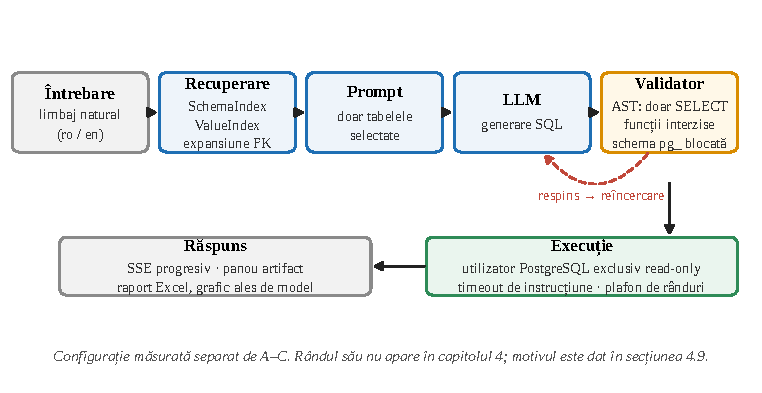
\includegraphics[width=\textwidth]{fig_arm_rag.pdf}
\caption{Configurația RAG: conducta proprie a sistemului. Recuperarea înlocuiește
schema integrală cu tabelele selectate, iar validarea pe arbore sintactic
precedă orice execuție.}
\label{fig:rag}
\end{figure}

\subsection{Configurația MCP — arhitectura agentică}
\label{sec:mcp}

Configurația agentică (figura~\ref{fig:mcp}) inversează raportul: modelul nu
primește nicio informație despre schemă în prompt, ci patru unelte expuse
printr-un server MCP peste transport stdio. Serverul este un strat subțire
de înregistrare a uneltelor peste un modul de acces la date fără dependențe
MCP, ceea ce permite testarea logicii de bază independent de protocol.

Bucla de decizie aparține integral modelului: acesta alege ce unelte apelează,
ordinea acestora și momentul în care dispune de informațiile necesare generării răspunsului. Consecința de
cost este structurală: la fiecare iterație întregul context
acumulat este retrimis, peste promptul de sistem al \emph{harness}-ului. Media
măsurată este între aproximativ 65\,000 și 162\,000 de tokeni de prompt per
întrebare, față de 1\,511 pentru un singur apel.

\begin{figure}[htbp]
\centering
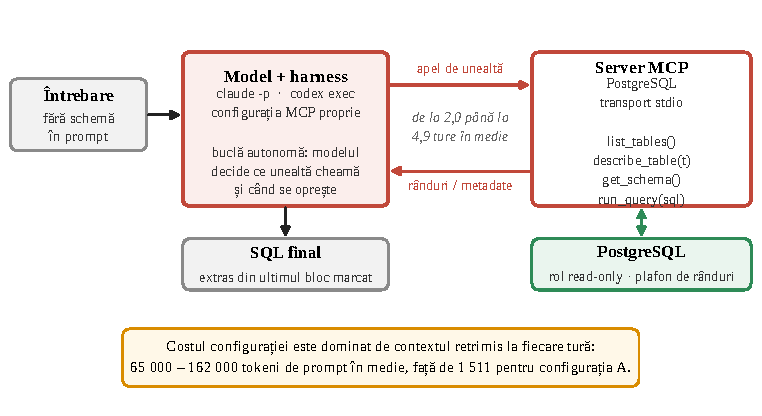
\includegraphics[width=\textwidth]{fig_arm_mcp.pdf}
\caption{Configurația agentică peste Model Context Protocol. Ceea ce se măsoară este
agentul \emph{așa cum este livrat}, cu promptul său de sistem implicit.}
\label{fig:mcp}
\end{figure}

\section{Cadrul de evaluare}
\label{sec:cadrul_evaluare}

\subsection{Structura}

Cadrul de evaluare (figura~\ref{fig:harness}) este organizat în jurul a trei
abstracții, fiecare izolând o sursă de eroare care, altfel, s-ar propaga în
rezultate.

\begin{figure}[htbp]
\centering
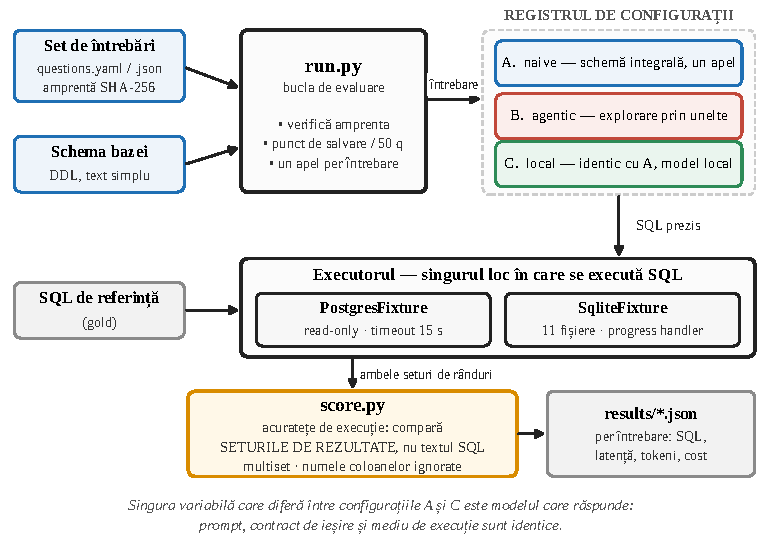
\includegraphics[width=\textwidth]{fig_harness.pdf}
\caption{Arhitectura cadrului de evaluare. Configurațiile diferă doar prin modul în
care se obține SQL-ul; execuția și punctarea sunt comune și identice pentru
toate.}
\label{fig:harness}
\end{figure}

\textbf{Registrul de configurații.} O configurație este o funcție cu semnătură unică:
primește o întrebare și returnează SQL-ul prezis împreună cu latența,
consumul de tokeni și eventualele erori. Sub această semnătură intră
deopotrivă un apel HTTP către un model din cloud, un subproces care
rulează un agent de linie de comandă și o cerere către un server local
llama.cpp. Bucla de evaluare este complet agnostică față de mecanismul concret de execuție utilizat.

\textbf{Executorul de interogări.} Este singurul loc în care se execută SQL,
atât cel de referință, cât și cel prezis. Existența lui este ceea ce permite
cadrului de evaluare să lucreze cu două motoare diferite: PostgreSQL pentru
primele două baze, SQLite pentru BIRD. Diferența nu este cosmetică. PostgreSQL
oferă \code{statement\_timeout}; SQLite nu are echivalent, așa că limita de
timp este impusă printr-un \emph{progress handler} apelat la fiecare 10\,000 de
instrucțiuni ale mașinii virtuale, care întrerupe execuția când termenul a
expirat. De asemenea, în cazul BIRD baza de date corectă este o proprietate
a \emph{întrebării}, nu a rulării, ceea ce a impus mutarea alegerii
conexiunii în interiorul executorului.

\textbf{Punctarea.} Modulul de punctare primește două seturi de rânduri și
returnează o valoare booleană. Nu vede niciodată textul SQL. Această
separare este cea care face imposibilă, prin construcție, o punctare bazată
pe asemănare textuală.

\subsection{Mecanisme de protecție împotriva rezultatelor false}

Trei mecanisme au fost adăugate special pentru a împiedica producerea unor
cifre plauzibile, dar greșite.

\emph{Amprentarea setului de întrebări.} Fiecare fișier de rezultate
conține amprenta setului de întrebări față de care a fost punctat. La generarea
tabelelor, un fișier cu amprentă diferită de cea curentă este semnalat ca
învechit și exclus, în loc să fie mediat în tăcere. Mecanismul a fost
verificat în practică: la generarea figurilor din capitolul~\ref{chap:rezultate} a fost
interceptată o rulare de 26 de întrebări din prima etapă, aflată în același
director cu rularea curentă de 44 de întrebări a aceluiași model.

\emph{Separarea erorilor de referință de erorile de model.} Interogarea de
referință și cea prezisă sunt executate separat, iar eșecurile sunt
înregistrate în câmpuri distincte. O interogare de referință care nu rulează
nu este contabilizată ca răspuns greșit al modelului.

\emph{Refuzul referințelor triviale.} Dacă o interogare de referință
returnează zero rânduri, rularea este oprită cu eroare. O referință vidă ar fi
validată de orice interogare care produce un rezultat vid, inclusiv de una
incorectă, introducând scoruri artificiale.

\subsection{Cele trei configurații măsurate}

Tabelul~\ref{tab:brate} prezintă definiția operațională a fiecăreia dintre cele trei configurații evaluate.

\begin{table}[H]
\centering
\caption{Definiția operațională a celor trei configurații.}
\label{tab:brate}
\footnotesize
\begin{tabularx}{\textwidth}{@{}p{2.1cm} L p{3.1cm}@{}}
\toprule
\hd{Configurație} & \hd{Ce primește modelul} & \hd{Cine conduce bucla} \\
\midrule
\textcolor{armA}{\textbf{A --- naiv}} &
Schema integrală ca text, un singur apel, instrucțiunea de a returna doar
SQL &
Procedură sincronă; apel unic \\
\textcolor{armB}{\textbf{B --- agentic}} &
Fără schemă inițială; explorare prin unelte MCP până la convergență &
Un agent de linie de comandă (\code{claude -p} \cite{claudecode},
\code{codex exec} \cite{codexcli}) sau configurația MCP proprie \\
\textcolor{armC}{\textbf{C --- local}} &
Prompt și contract \emph{identice} cu A; diferă doar modelul &
Procedură sincronă; apel unic prin llama.cpp pe GPU local \\
\bottomrule
\end{tabularx}
\end{table}

Identitatea dintre A și C este deliberată și este ceea ce face comparația
interpretabilă: un rând local și unul din cloud diferă printr-o singură
variabilă.

\section{Bazele de date și seturile de întrebări}
\label{sec:baze_date}

Măsurătorile folosesc trei baze de date de dimensiuni și proveniențe
diferite, alese astfel încât rezultatul să nu depindă de o singură schemă.
Tabelul~\ref{tab:baze} sintetizează caracteristicile acestor baze de date și numărul de întrebări asociate.

\begin{table}[H]
\centering
\caption{Cele trei baze de date de evaluare și seturile de întrebări
asociate. Dimensiunea promptului este numărul de caractere al schemei
transmise modelului în configurația A, măsurat din fișierele de rezultate.}
\label{tab:baze}
\footnotesize
\begin{tabularx}{\textwidth}{@{}p{2.5cm} R R R R L@{}}
\toprule
\hd{Baza} & \hd{Tabele} & \hd{Coloane} & \hd{Rânduri} & \hd{Schemă (car.)}
& \hd{Întrebări} \\
\midrule
\code{car\_rental} & 9 & $\approx$70 & 8\,026 & 5\,951 &
51: 44 punctate + 7 ambigue \\
\code{adventureworks} & 68 & 455 & $\approx$761\,000 & 37\,019 &
56: 49 punctate + 7 ambigue \\
BIRD-SQL dev & 75 & 798 & 3\,932\,735 & variabilă &
1\,534, toate punctate \\
\midrule
\multicolumn{6}{@{}l@{}}{\footnotesize BIRD-SQL dev însumează 11 baze SQLite
distincte, de la 3 la 13 tabele fiecare, 1,49 GB pe disc.} \\
\bottomrule
\end{tabularx}
\end{table}

\code{car\_rental} este baza demonstrativă a sistemului: mică, cu schemă
curată, folosită pentru a izola dificultatea SQL de dificultatea schemei.
\code{adventureworks} este baza de date OLTP demonstrativă publicată de Microsoft \cite{advworks}, cu 68 de
tabele de bază, 455 de coloane, 91 de chei străine și cinci scheme; o schemă de 37\,019 caractere
testează dacă avantajul configurației A rezistă când promptul crește de șase ori.
BIRD-SQL dev \cite{bird} introduce un element absent din primele două baze: un set de întrebări
elaborate independent de autorul lucrării. Setul este construit din două artefacte distincte,
care nu sunt distribuite împreună: revizia de întrebări și interogări de
referință \cite{birddata} și pachetul celor 11 baze SQLite; asocierea lor,
împreună cu validarea fiecărei interogări de referință, este făcută de un
script dedicat (anexa~\ref{anx:reproducere}).

\subsection{Categoriile de întrebări}
\label{sec:categorii}

Cele două seturi proprii sunt construite pe
categorii derivate din taxonomia de erori din Spider 2.0 \cite{spider2} și
din analiza de eșecuri a BIRD \cite{bird}. Distribuția este dată în
tabelul~\ref{tab:categorii}.

\begin{table}[H]
\centering
\caption{Distribuția întrebărilor pe categorii. Grupurile marcate cu
$\dagger$ au fost adăugate în etapa a doua, după ce categoriile inițiale au
încetat să diferențieze sistemele.}
\label{tab:categorii}
\footnotesize
\begin{tabularx}{\textwidth}{@{}p{2.6cm} L R R@{}}
\toprule
\hd{Grup} & \hd{Ce conține} & \hd{car\_rental} & \hd{advent.} \\
\midrule
simple & selecție și filtrare pe o tabelă & 6 & 5 \\
agregare & \code{GROUP BY}, funcții de agregare & 9 & 8 \\
join & îmbinări pe două sau mai multe tabele & 5 & 10 \\
subinterogare & subinterogări corelate și necorelate & 6 & 7 \\
fereastră$\dagger$ & funcții fereastră, cadre explicite & 5 & 5 \\
structură$\dagger$ & agregare pe mai multe niveluri, auto-îmbinare,
anti-îmbinare, recursivitate, operații pe mulțimi, goluri și insule (\emph{gaps and islands}) & 5 & 7 \\
măsură$\dagger$ & rapoarte, percentile, pivotare & 4 & 3 \\
temporal$\dagger$ & aritmetică de calendar, cohorte & 4 & 4 \\
\midrule
ambigue & fără răspuns unic; punctate separat & 7 & 7 \\
\bottomrule
\end{tabularx}
\end{table}

Categoria \emph{ambiguă} necesită o precizare metodologică distinctă, fiind singura evaluată
după un criteriu calitativ. Aceste întrebări nu admit un răspuns SQL unic. De exemplu,
„Care este venitul mediu per client?” permite trei interpretări valide în schema \code{car\_rental}.
Sistemul este evaluat nu pe baza interogării emise, ci pe capacitatea de a \emph{solicita clarificări}
în loc de a selecta arbitrar o interpretare implicită. Patru dintre cele paisprezece
întrebări sunt formulate în limba română, pentru a verifica dacă
comportamentul se transferă între limbi.

\section{Alegerea tehnologiilor}

\begin{itemize}[nosep,leftmargin=*]
  \item \textbf{PostgreSQL} \cite{postgresql} \textbf{prin \code{pgserver}} \cite{pgserver}: executorul pornește o
    instanță PostgreSQL încorporată, fără Docker și fără instalare de sistem.
    Este condiția practică pentru ca rezultatele să fie reproductibile de un
    evaluator extern.
  \item \textbf{SQLite} \cite{sqlite} pentru BIRD — interogările de referință ale BIRD sunt
    scrise pentru SQLite. Portarea lor la PostgreSQL ar fi însemnat
    înlocuirea SQL-ului setului de evaluare cu SQL propriu, adică modificarea
    obiectului măsurat. A fost adăugat în schimb un executor SQLite.
  \item \textbf{llama.cpp} \cite{llamacpp} pentru configurația locală, expus prin interfața
    compatibilă OpenAI, ceea ce permite configurațiilor A și C să folosească
    exact același cod client.
  \item \textbf{Agenți de linie de comandă ca subprocese}: configurația B rulează
    agenții \emph{așa cum sunt livrați}, cu promptul lor de sistem implicit.
    Ceea ce se măsoară este comportamentul real al produsului.
\end{itemize}

% =====================================================================
\chapter{Testarea soluției și rezultate experimentale}
\label{chap:rezultate}
% =====================================================================

Acest capitol prezintă protocolul de măsurare și rezultatele obținute.
Structura urmează logica experimentului: mai întâi condițiile în care s-a
măsurat (secțiunea~\ref{sec:metodologie_testare}), apoi rezultatul de ansamblu (secțiunea~\ref{sec:rezultat_ansamblu}), apoi fiecare configurație în parte
(secțiunile~\ref{sec:config_a}--\ref{sec:config_c}), apoi analizele care explică factorii
determinanți ai rezultatelor obținute (secțiunile~\ref{sec:dificultate}--\ref{sec:ambiguitate}), apoi validarea externă (secțiunea~\ref{sec:bird}) și, în final, limitele
măsurătorii (secțiunea~\ref{sec:validitate}).

\section{Metodologia de testare}
\label{sec:metodologie_testare}

\subsection{Punerea în funcțiune}

Cadrul de evaluare nu necesită instalare de sistem. Executorul PostgreSQL pornește
o instanță încorporată prin \code{pgserver}, iar baza este creată din
scripturile de inițializare la prima rulare. Modelele locale sunt servite de
llama.cpp prin interfața compatibilă OpenAI. Cheia de acces pentru modelele
din cloud este citită din mediu. O rulare completă se lansează cu o singură
comandă (anexa~\ref{anx:reproducere}).

\subsection{Parametrii de testare}

Parametrii ficși ai tuturor măsurătorilor sunt sintetizați în tabelul~\ref{tab:param}.

\begin{table}[H]
\centering
\caption{Parametrii ficși ai tuturor măsurătorilor.}
\label{tab:param}
\footnotesize
\begin{tabularx}{\textwidth}{@{}p{4.4cm} L@{}}
\toprule
\hd{Parametru} & \hd{Valoare} \\
\midrule
Metrică & acuratețe de execuție; comparare de multimulțimi de tupluri;
numele coloanelor ignorate; ordinea contează doar dacă întrebarea o cere \\
Temperatură & 0 pentru toate modelele \\
Repetări & o rulare per celulă (vezi limitele din secțiunea~\ref{sec:validitate}) \\
Timp maxim per instrucțiune & 15 s, impus în executor \\
Context / buget de ieșire, configurație C & 16\,384 / 8\,192 tokeni \\
Hardware, configurație C & RTX 5070, 12 GiB VRAM; 31 GiB RAM; i9-14900K \\
Motor de inferență, configurație C & llama.cpp, compilare CUDA \code{cb295bf} \\
Preț de referință & tarife verificate la 23.08.2026, înregistrate în
fiecare fișier de rezultate \\
\bottomrule
\end{tabularx}
\end{table}

\subsection{Criterii de evaluare și punctare}

Din cele 51 de întrebări \code{car\_rental}, 44 sunt punctate pe acuratețe și 7
sunt ambigue, punctate separat (vezi secțiunea~\ref{sec:ambiguitate}). Aceeași separare se aplică la
\code{adventureworks} (49 + 7). Toate procentele de acuratețe din acest
capitol se raportează la populația punctată, iar numărătorile de erori din
tabelele configurației C se raportează la aceeași populație: o precizare
necesară, deoarece raportarea acelorași erori la întregul set de 51 de întrebări
ar genera valori procentuale diferite.

O rulare a fost exclusă integral. \code{claude-agent} pe \code{claude-fable-5}
a atins limita de utilizare a contului la întrebarea 41; pentru ultimele 11
întrebări procesul a ieșit imediat cu eroare. Scorul brut de 75,0\,\% al
acestui fișier clasifică 8 eșecuri de infrastructură drept răspunsuri eronate,
motiv pentru care rularea \textbf{a fost exclusă din analiza comparativă}. Nicio altă rulare nu a avut vreun eșec de
infrastructură.

\section{Rezultatul de ansamblu}
\label{sec:rezultat_ansamblu}

Figura~\ref{fig:headline} prezintă toate cele 18 rulări: cinci modele din
cloud cu un singur apel, șapte configurații agentice și șase modele
rulate local, măsurate pe
\code{car\_rental}, colorate după configurație.

\begin{figure}[htbp]
\centering
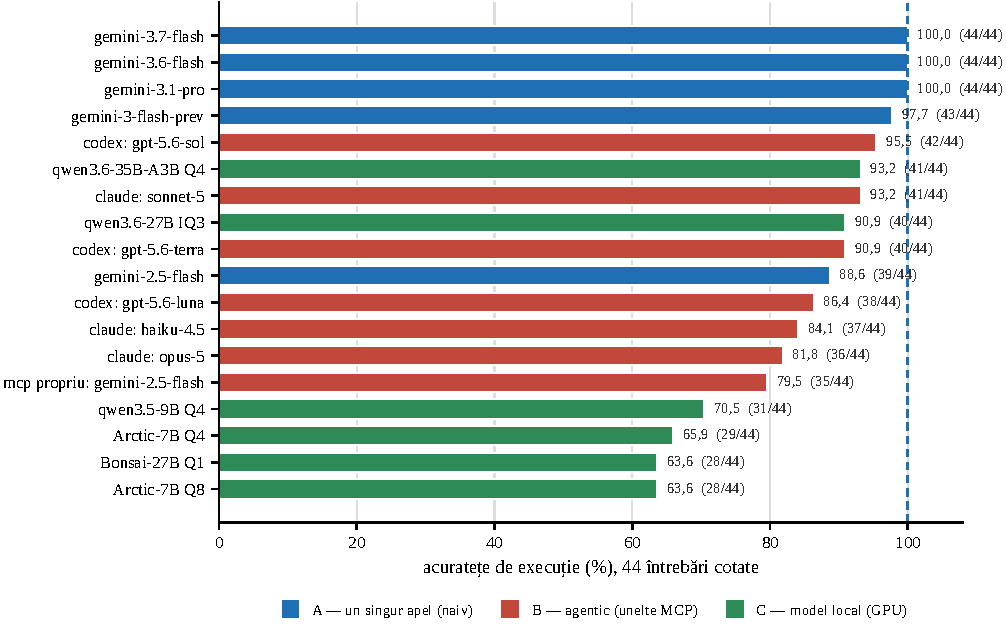
\includegraphics[width=0.98\textwidth]{fig_accuracy_arms.pdf}
\caption{Acuratețea de execuție a tuturor sistemelor măsurate pe
\code{car\_rental}, 44 de întrebări punctate. Linia întreruptă marchează
plafonul atins de configurația A. Niciun sistem agentic nu îl atinge.}
\label{fig:headline}
\end{figure}

Din analiza datelor reies trei observații principale:

\begin{enumerate}[nosep,leftmargin=*]
  \item \textbf{Primele patru sisteme din clasament folosesc toate
    configurația A}, cea mai simplă dintre cele trei. Cel mai bun sistem
    agentic răspunde corect la 42 din cele 44 de întrebări, reprezentând
    o performanță notabilă; totuși, trei configurații cu un singur apel
    ating scorul maxim de 44/44.
  \item \textbf{Un model local de 35 de miliarde de parametri, rulat pe o
    placă de 12 GiB, obține 93,2\,\%}, exact scorul celui mai bun agent din
    familia Claude, fără ca datele să părăsească infrastructura locală.
  \item \textbf{Ordinea nu urmează capacitatea modelelor.} În configurația agentică,
    modelul cel mai puternic al familiei Claude (Opus 5, 81,8\,\%) se
    clasează sub cel mediu (Sonnet 5, 93,2\,\%) și sub cel mic (Haiku 4.5,
    84,1\,\%). Acest tipar reapare independent (vezi secțiunea~\ref{sec:bird}).
\end{enumerate}

\section{Configurația A --- un singur apel}
\label{sec:config_a}

\begin{table}[H]
\centering
\caption{Configurația A: schema integrală, un apel. Costul este extrapolat din
consumul de tokeni măsurat, la tarifele verificate la 23.08.2026.}
\label{tab:naive}
\footnotesize
\begin{tabular}{@{}lrrrrrr@{}}
\toprule
 & \multicolumn{2}{c}{\hd{Acuratețe}} & \multicolumn{4}{c}{\hd{Măsurat pe car\_rental}} \\
\cmidrule(lr){2-3}\cmidrule(l){4-7}
\hd{Model} & \hd{car\_rental} & \hd{AdventureWorks} & \hd{Latență med.} & \hd{Tok.\ prompt} & \hd{Tok.\ ieșire} & \hd{\$/100 î.} \\
\midrule
\code{gemini-3.7-flash} & 100,0\,\% & 100,0\,\% & 2,7\,s & 1\,511 & 685 & \$0,37 \\
\code{gemini-3.6-flash} & 100,0\,\% & 98,0\,\% & 6,4\,s & 1\,511 & 1\,079 & \$0,52 \\
\code{gemini-3.1-pro} & 100,0\,\% & 100,0\,\% & 6,7\,s & 1\,511 & 1\,470 & \$2,07 \\
\code{gemini-3-flash-prev} & 97,7\,\% & 98,0\,\% & 4,4\,s & 1\,511 & 1\,547 & \$0,54 \\
\code{gemini-2.5-flash} & 88,6\,\% & 91,8\,\% & 1,9\,s & 1\,511 & 654 & \$0,21 \\
\bottomrule
\end{tabular}

\end{table}

Rezultatele obținute de configurația A sunt sintetizate în tabelul~\ref{tab:naive}.
Setul curent de întrebări separă decisiv \code{gemini-2.5-flash} și diferențiază
ușor cele două modele intermediare, dar trei din cinci modele obțin în continuare
scorul maxim. Diferența dintre generații este reală și mare: de la
\code{gemini-2.5-flash} la \code{gemini-3.7-flash} sunt +11,4 puncte
procentuale pe \code{car\_rental}, la un preț comparabil.

Un rezultat esențial pentru interpretarea capitolului este că extinderea schemei de la 5\,951 la
37\,019 caractere (de peste șase ori) \emph{nu} degradează performanța configurației A.
Cele două modele de vârf își mențin acuratețea de 100\,\% pe ambele baze de date.
Ipoteza conform căreia transmiterea schemei integrale nu este scalabilă nu se verifică
empiric la acest ordin de mărime al schemei.

\section{Configurația B --- agentic}
\label{sec:config_b}

Sunt măsurate două tipuri de sisteme. Primele șase rânduri din
tabelul~\ref{tab:agentic} sunt agenți de programare comerciali, rulați ca
atare peste serverul MCP al proiectului. Ultimul rând este bucla proprie: un
client minimal scris pentru această lucrare, care trimite întrebarea modelului
\code{gemini-2.5-flash}, execută uneltele pe care acesta le cere și îi
returnează rezultatele, până când modelul produce interogarea finală. Nu are
prompt de sistem elaborat și nici strategie de explorare proprie.

Acest rând permite singura comparație complet controlată din capitol.
\code{gemini-2.5-flash} este măsurat și în configurația A, pe aceleași 44 de
întrebări și cu aceeași punctare, unde obține 88,6\,\%. Prin unelte, același
model obține 79,5\,\%. \textbf{Diferența de 9,1 puncte este atribuibilă
exclusiv arhitecturii}, fiindcă modelul, întrebările și baza de date sunt
identice. Restul rândurilor din tabel amestecă efectul arhitecturii cu cel al
modelului și al agentului comercial care îl conduce.

\begin{table}[H]
\centering
\caption{Configurația agentică, \code{car\_rental}. Costurile Claude sunt cifrele
proprii ale \emph{harness}-ului, care țin cont de memorarea contextului; la tarif
de listă, Sonnet ar costa \$33,35 și Opus \$66,49 la 100 de întrebări.}
\label{tab:agentic}
\footnotesize
\setlength{\tabcolsep}{4pt}
\begin{tabular}{@{}lrrrrrr@{}}
\toprule
\hd{Sistem} & \hd{Corecte} & \hd{Acuratețe} & \hd{Iterații med.} & \hd{Latență med.} & \hd{Tok.\ prompt} & \hd{\$/100 î.} \\
\midrule
\code{codex: gpt-5.6-sol} & 42/44 & \textbf{95,5\,\%} & 2,3 & 23,6\,s & 67\,848 & nepublicat \\
\code{claude: sonnet-5} & 41/44 & \textbf{93,2\,\%} & 4,4 & 12,4\,s & 162\,170 & \$9,44 \\
\code{codex: gpt-5.6-terra} & 40/44 & \textbf{90,9\,\%} & 2,1 & 18,0\,s & 64\,916 & nepublicat \\
\code{codex: gpt-5.6-luna} & 38/44 & \textbf{86,4\,\%} & 2,5 & 22,0\,s & 70\,978 & nepublicat \\
\code{claude: haiku-4.5} & 37/44 & \textbf{84,1\,\%} & 4,2 & 18,2\,s & 100\,572 & \$3,33 \\
\code{claude: opus-5} & 36/44 & \textbf{81,8\,\%} & 5,0 & 18,0\,s & 126\,673 & \$23,19 \\
\code{mcp propriu: gemini-2.5-flash} & 35/44 & \textbf{79,5\,\%} & 2,5 & 4,8\,s & nemăsurat & nemăsurat \\
\midrule
\emph{referință:} configurația A, cea mai bună & 44/44 & \textbf{100,0\,\%} & 0 & 2,7\,s & 1\,511 & \$0,37 \\
\bottomrule
\end{tabular}

\end{table}

\subsection{Eficiența accesului prin unelte în raport cu linia de referință}

Toate configurațiile agentice măsurate răspund corect la majoritatea
întrebărilor (între 79,5\,\% și 95,5\,\%), deci accesul la baza de
date prin unelte este o abordare care funcționează. Niciuna nu atinge însă
reperul obținut cu un singur apel, iar diferența nu este marginală: 4,5
puncte pentru cel mai bun agent și 20,5 puncte pentru cel mai slab. Rezultatul
se reproduce peste \textbf{două \emph{harness}-uri complet diferite}
(\code{claude -p} \cite{claudecode} și \code{codex exec}
\cite{codexcli}), peste \textbf{șase modele} de la doi furnizori, plus
configurația MCP proprie a proiectului, construită peste un al treilea
furnizor. Nu este, prin urmare, o particularitate a unei implementări.

Explicația plauzibilă este aceea că arhitectura B nu măsoară capacitatea modelului, ci
interacțiunea dintre comportamentul implicit al unui \emph{harness} de
programare și o sarcină de explorare a schemei. Un agent proiectat să
exploreze temeinic un depozit de cod explorează temeinic și o bază de date,
consumă din bugetul de atenție pe rezultate intermediare și ajunge la
formularea interogării cu un context deja încărcat. Observația care susține
această interpretare este că \emph{modelul cel mai capabil consumă cele mai
multe iterații} --- Opus 5, cu 5,0 iterații în medie, este ultimul dintre modelele
comerciale din această configurație.

\subsection{Costul}

\begin{figure}[htbp]
\centering
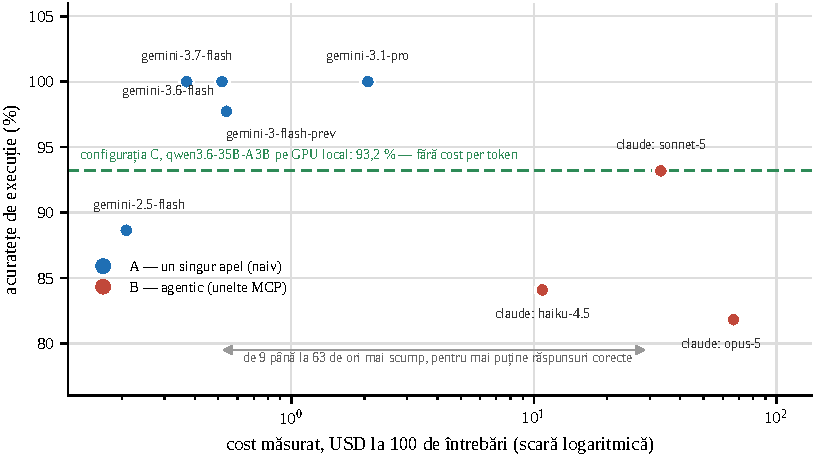
\includegraphics[width=0.95\textwidth]{fig_cost_accuracy.pdf}
\caption{Costul măsurat în raport cu acuratețea de execuție. Configurațiile se diferențiază pe axa costului
cu peste un ordin de mărime, în defavoarea abordării agentice.}
\label{fig:cost}
\end{figure}

Așa cum ilustrează figura~\ref{fig:cost}, costul separă configurațiile mult mai puternic decât acuratețea: \$0,37 la
100 de întrebări pentru un singur apel, față de \$3,33--\$23,19 pentru
variantele agentice: \textbf{un factor de cost de 9 până la 63 de ori mai mare, asociat
unei rate inferioare de răspunsuri corecte}. Cauza este coloana de tokeni de prompt: 65\,000
până la 162\,000 în medie, față de 1\,511, fiindcă un agent retrimite
întregul context la fiecare iterație, peste promptul de sistem al \emph{harness}-ului.

Rezultatele experimentale nu implică o deficiență intrinsecă a modelelor agentice;
interpretarea susținută de date este că un agent generalist de programare
nu reprezintă instrumentul optim pentru o sarcină deterministă, rezolvabilă
mai eficient printr-un apel unic bine structurat. Distincția nu poate fi însă tranșată de acest experiment, care
compară sisteme întregi, nu componente izolate.

\section{Configurația C --- modele rulate local}
\label{sec:config_c}

\subsection{Acuratețea}

\begin{table}[H]
\centering
\caption{Configurația C: modele rulate local. Coloanele de eșecuri se
raportează la cele 44 de întrebări punctate.}
\label{tab:localacc}
\footnotesize
\begin{tabular}{@{}lllrrr@{}}
\toprule
 & \multicolumn{2}{c}{\hd{Acuratețe}} & \multicolumn{3}{c}{\hd{Eșecuri pe car\_rental}} \\
\cmidrule(lr){2-3}\cmidrule(l){4-6}
\hd{Model} & \hd{car\_rental} & \hd{AdventureWorks} & \hd{SQL inv.} & \hd{fără SQL} & \hd{trunchiat} \\
\midrule
\code{qwen3.6-35B-A3B Q4} & \textbf{93,2\,\%} (41/44) & 85,7\,\% (42/49) & 2 & 0 & 0 \\
\code{qwen3.6-27B IQ3} & \textbf{90,9\,\%} (40/44) & nerulat & 3 & 0 & 0 \\
\code{qwen3.5-9B Q4} & \textbf{70,5\,\%} (31/44) & 67,3\,\% (33/49) & 0 & 5 & 5 \\
\code{Arctic-7B Q4} & \textbf{65,9\,\%} (29/44) & 55,1\,\% (27/49) & 10 & 0 & 0 \\
\code{Bonsai-27B Q1} & \textbf{63,6\,\%} (28/44) & 69,4\,\% (34/49) & 6 & 6 & 6 \\
\code{Arctic-7B Q8} & \textbf{63,6\,\%} (28/44) & 55,1\,\% (27/49) & 9 & 0 & 0 \\
\bottomrule
\end{tabular}

\end{table}

Rezultatele privind acuratețea sunt prezentate în tabelul~\ref{tab:localacc}.
Rezultatul principal al acestei configurații este primul rând: un model MoE de 35 de
miliarde de parametri, cuantizat pe 4 biți, atinge 93,2\,\% pe
\code{car\_rental} --- egal cu cel mai bun agent Claude --- și 85,7\,\% pe o
schemă de 68 de tabele. Pentru un sistem care prelucrează date de
întreprindere, echivalența funcțională cu un serviciu din cloud, obținută
fără ca datele să părăsească infrastructura locală, reprezintă o concluzie cu consecințe practice
directe.

\subsection{Constrângerea de performanță: modele dense versus MoE}

\begin{table}[H]
\centering
\caption{Configurația C: încadrarea în memoria plăcii și consecința asupra
debitului. VRAM este ocuparea măsurată la încărcare.}
\label{tab:localperf}
\footnotesize
\begin{tabular}{@{}lrrlrrr@{}}
\toprule
\hd{Model} & \hd{GGUF (GiB)} & \hd{VRAM (MiB)} & \hd{Cum încape} & \hd{tok/s} & \hd{Latență med.} & \hd{Durată, 44 î.} \\
\midrule
Arctic-7B Q4 & 4,4 & 6\,055 & rezident integral & 113 & 4,0\,s & 4 min \\
qwen3.5-9B Q4 & 5,2 & 6\,702 & rezident integral & 91 & 8,7\,s & 15 min \\
Arctic-7B Q8 & 7,5 & 9\,067 & rezident integral & 72 & 6,1\,s & 5 min \\
Bonsai-27B Q1 & 3,5 & 6\,284 & rezident integral & 53 & 47,2\,s & 50 min \\
\textbf{qwen3.6-35B-A3B Q4} & 20,6 & 9\,620 & experți în RAM & \textbf{50} & 39,5\,s & 37 min \\
qwen3.6-27B IQ3 & 11,2 & 10\,438 & straturi parțiale & 8 & 268,5\,s & 247 min \\
\bottomrule
\end{tabular}

\end{table}

În tabelul~\ref{tab:localperf} sunt sintetizate ocuparea memoriei și debitele de generare obținute.
Ultimele două rânduri evidențiază o discrepanță arhitecturală remarcabilă.
Modelul cu \emph{cel mai mare volum ocupat pe disc} (20,6 GiB, depășind capacitatea
de 12 GiB a memoriei VRAM) atinge un debit de generare de 50 tokeni/secundă, în timp
ce un model dens de dimensiune aproximativ la jumătate (11,2 GiB) obține doar 8 tokeni/secundă.
Modelul MoE este \textbf{de peste șase ori mai rapid} și, totodată, mai exact
(93,2\,\% față de 90,9\,\%).

\begin{figure}[htbp]
\centering
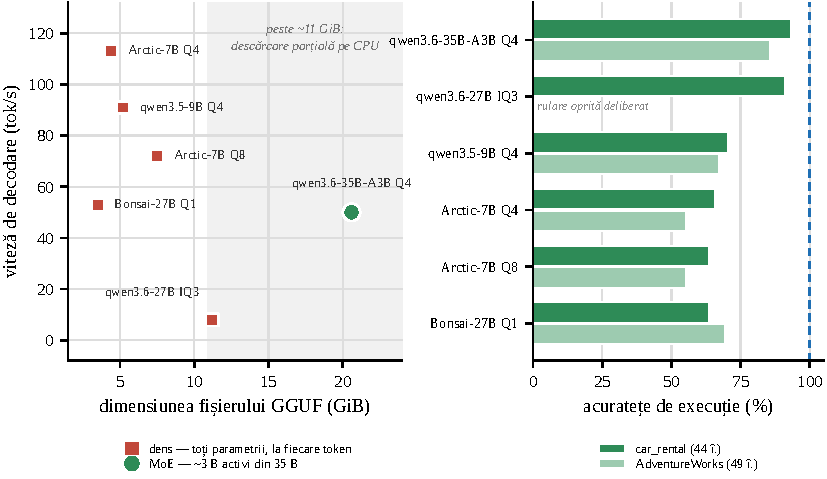
\includegraphics[width=\textwidth]{fig_local.pdf}
\caption{Stânga: debitul de decodare nu este o funcție descrescătoare de
dimensiunea fișierului. Punctul verde este singurul model MoE. Dreapta:
acuratețea acelorași modele pe cele două baze PostgreSQL.}
\label{fig:local}
\end{figure}

Comportamentul este ilustrat în figura~\ref{fig:local}. Explicația este arhitecturală.
Un model dens citește toți parametrii pentru
fiecare token generat; când nu încape în VRAM, aproximativ 5 GiB traversează
magistrala PCIe \emph{la fiecare token}. Un model MoE citește doar
aproximativ 3 din cei 35 de miliarde de parametri, ceea ce permite păstrarea
experților inactivi în memoria RAM a sistemului cu o penalizare redusă de latență. Pe sisteme cu resurse hardware limitate,
\textbf{criteriul de selecție nu este dimensiunea statică a modelului, ci volumul de parametri
transferat per token generat}.

Consecința practică este că modelul dens de 27B nu este o configurație
utilizabilă pentru un sistem interactiv, \emph{la orice acuratețe}: 247 de
minute pentru 44 de întrebări înseamnă aproximativ 5,6 minute per întrebare.

\subsection{Rezultate experimentale secundare}

\textbf{Cuantizarea nu explică diferențele de acuratețe.}
Arctic-Text2SQL-R1 a fost măsurat de două ori, cu aceleași greutăți: varianta
pe 8 biți (7,5 GiB) obține un scor \emph{mai mic} decât cea pe 4 biți
(4,4 GiB) pe \code{car\_rental} (63,6\,\% față de 65,9\,\%) și identic
pe AdventureWorks, rulând totodată la 64\,\% din viteză. Dublarea numărului
de biți nu a adus niciun beneficiu.

\textbf{Problema modelului specializat este dialectul, nu raționamentul.}
Din cele 10 erori de execuție ale modelului Arctic pe \code{car\_rental},
\textbf{8 sunt funcții SQLite pe care PostgreSQL nu le are} ---
\code{strftime} (de cinci ori), \code{date(...)} folosit ca constructor (de
două ori) și \code{julianday}. Numărul este o limită inferioară: clasificarea
se face după numele funcției, așa că o a noua eroare, \code{operator does not
exist: date - bigint} (aritmetică de tip dată minus întreg, tot o
particularitate SQLite) nu este numărată. Modelul a fost antrenat pe Spider și
BIRD, ambele livrate în SQLite, și emite funcții de dată SQLite în ciuda unui
prompt care specifică explicit „PostgreSQL” și a unei scheme redate în tipuri PostgreSQL.
Dacă fiecare astfel de eșec ar fi rescris mecanic în echivalentul PostgreSQL,
modelul ar ajunge la 84,1\,\%. Această valoare arată cât din decalaj se
explică prin dialect și \emph{nu este un scor obținut de model}: acuratețea
lui măsurată rămâne 65,9\,\%.

Aceasta este o observație cu valoare generală: \textbf{o poziție în clasament
nu se transferă între motoare de baze de date}. Eticheta „model specializat”
descrie un dialect la fel de mult ca o sarcină: aspect ce nu este evidențiat în
clasamentele majore, deoarece acestea evaluează predominant pe dialectul SQLite.

\section{Analiza factorilor de dificultate}
\label{sec:dificultate}

\begin{table}[H]
\centering
\caption{Acuratețea agregată pe grupuri de întrebări, \code{car\_rental},
mediată peste toate rulările fiecărei familii de configurații (\%).}
\label{tab:categorii-rez}
\footnotesize
\begin{tabular}{@{}lrrrrrrrr@{}}
\toprule
\hd{Familie} & \hd{simple} & \hd{agreg.} & \hd{join} & \hd{subint.} & \hd{fereastră} & \hd{structură} & \hd{măsură} & \hd{temporal} \\
\midrule
A --- un singur apel & 100,0 & 100,0 & 100,0 & 100,0 & 96,0 & 92,0 & 95,0 & 90,0 \\
B --- agentic & 95,2 & 87,3 & 85,7 & 78,6 & 85,7 & 85,7 & 92,9 & 89,3 \\
C --- local & 97,2 & 94,4 & 86,7 & 80,6 & 60,0 & 43,3 & 70,8 & 33,3 \\
\bottomrule
\end{tabular}

\end{table}

\begin{figure}[htbp]
\centering
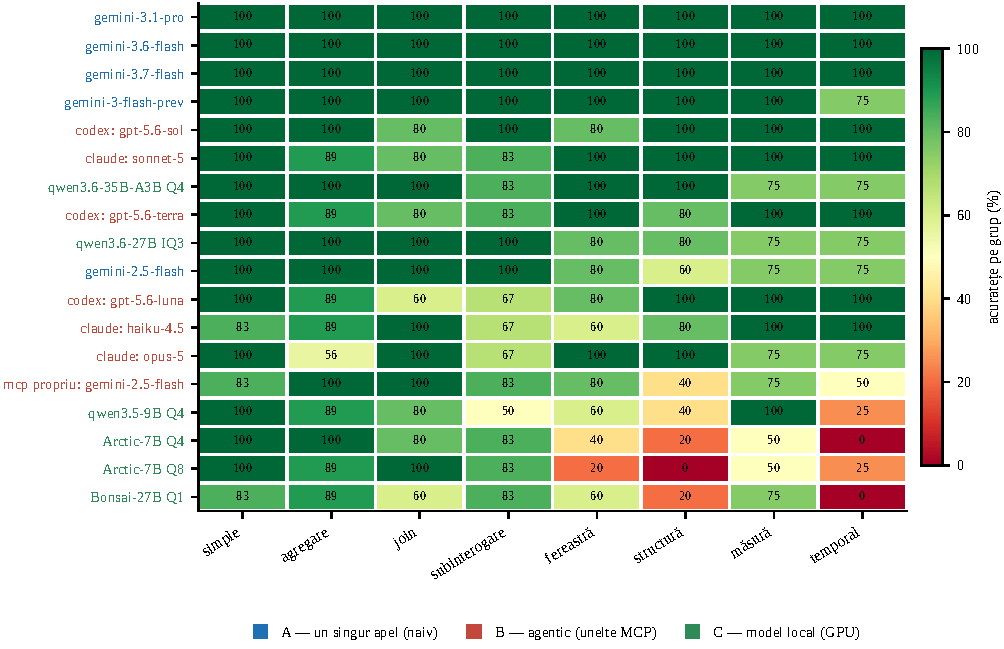
\includegraphics[width=0.96\textwidth]{fig_categories.pdf}
\caption{Acuratețea pe grupuri de întrebări, per sistem. Culoarea etichetei
indică configurația. Categoriile din stânga prezintă un grad ridicat de saturație,
în timp ce categoriile din dreapta evidențiază o capacitate puternică de discriminare.}
\label{fig:categorii}
\end{figure}

Tabelul~\ref{tab:categorii-rez} și figura~\ref{fig:categorii} ilustrează aceleași concluzii
din două perspective complementare. Grupurile
\emph{simple} și \emph{agregare} (exact cele pe care le conțin seturile
de evaluare clasice) nu mai separă niciun sistem din configurațiile A și B. Puterea
de discriminare s-a mutat în cea mai mare parte în grupurile
adăugate în etapa a doua: configurația locală scade de la 97,2\,\% pe \emph{simple}
la 43,3\,\% pe \emph{structură} și 33,3\,\% pe \emph{temporal}. Excepția o
constituie configurația agentică, care pierde cel mai mult pe \emph{subinterogare}
(78,6\,\%), o categorie din prima etapă: ceea ce confirmă observația din
secțiunea~\ref{sec:config_b}, că această configurație nu eșuează pe aceleași dimensiuni ca celelalte
două.

Aceasta este și dovada că întrebările adăugate testează ceea ce au fost
proiectate să testeze: fiecare punct pe care îl pierde
\code{gemini-2.5-flash} se află într-unul dintre grupurile noi, iar cele
patru categorii inițiale rămân răspunse perfect.

Inspecția manuală a interogărilor greșite, peste toate rulările, identifică
trei moduri de eșec recurente, detaliate în tabelul~\ref{tab:esecuri}:

\begin{table}[H]
\centering
\caption{Modurile de eșec recurente, identificate prin reexecutarea manuală a
interogărilor greșite.}
\label{tab:esecuri}
\footnotesize
\begin{tabularx}{\textwidth}{@{}p{3.6cm} L@{}}
\toprule
\hd{Mod de eșec} & \hd{Descrierea manifestării} \\
\midrule
Semantica cadrului de fereastră &
Filtrarea pe anul de raportare este aplicată \emph{înainte} de funcția
fereastră, ceea ce trunchiază cadrul peste care se calculează \\
Utilizarea greșită a dialectului &
\code{round(double precision, integer) does not exist} --- în PostgreSQL,
varianta cu două argumente cere \code{numeric}. Este exact a doua subclasă
de erori ca frecvență din Spider 2.0 (10,3\,\%) \cite{spider2} \\
Ancorarea cohortei &
Cohorta este ancorată la data evenimentului greșit: cazul de eșec
emblematic din Spider 2.0 \\
\bottomrule
\end{tabularx}
\end{table}

\section{Ambiguitatea, singura dimensiune nesaturată}
\label{sec:ambiguitate}

Cele șapte întrebări ambigue nu au un răspuns corect. Sistemul este punctat pe
faptul dacă \emph{a cerut} o clarificare, rezultatele fiind sintetizate în tabelul~\ref{tab:ambig} și figura~\ref{fig:ambig}.

\begin{table}[H]
\centering
\caption{Câte rulări din fiecare familie au cerut clarificare, per întrebare,
\code{car\_rental}. Cinci rulări cu un singur apel, șapte agentice, șase
locale.}
\label{tab:ambig}
\footnotesize
\begin{tabularx}{\textwidth}{@{}llrrr@{}}
\toprule
\hd{Î.} & \hd{Textul întrebării} & \hd{Config. A} & \hd{Config. B} & \hd{Config. C} \\
\midrule
\code{q30} & \emph{„Hello, what can you do?”} & 5/5 & 4/7 & 6/6 \\
\code{q28} & \emph{„Show me the good vehicles.”} & 4/5 & 6/7 & 2/6 \\
\code{q29} & \emph{„How is the business doing?”} & 3/5 & 4/7 & 1/6 \\
\code{q27} & \emph{„Care sunt cei mai buni clienți?”} & 1/5 & 4/7 & 1/6 \\
\code{q49} & \emph{„Care sucursală a adus cei mai mulți bani în 2024?”} & \textbf{0/5} & 3/7 & 1/6 \\
\code{q51} & \emph{„How many cars were rented last month?”} & \textbf{0/5} & 3/7 & \textbf{0/6} \\
\code{q50} & \emph{„What is our average revenue per client?”} & \textbf{0/5} & 2/7 & \textbf{0/6} \\
\bottomrule
\end{tabularx}

\end{table}

\begin{figure}[htbp]
\centering
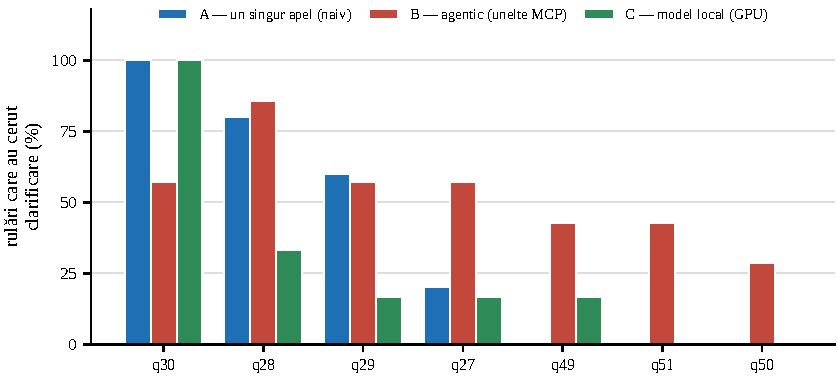
\includegraphics[width=0.95\textwidth]{fig_ambiguity.pdf}
\caption{Rata de solicitare a clarificării, pe întrebare și pe familie de
configurații. Ordinea pe axa orizontală este descrescătoare după rata medie.}
\label{fig:ambig}
\end{figure}

Din aceste măsurători se desprind trei concluzii metodologice esențiale:

\textbf{1. Ambiguitatea care se anunță este detectată; cea care se ascunde nu
este.} O întrebare care nu conține nicio metrică („Cum merge afacerea?”)
declanșează o cerere de clarificare. O întrebare care \emph{pare}
răspunzabilă nu o declanșează. „Care este venitul mediu per client?” admite
trei numitori apărabili în această schemă, iar \textbf{toate cele cinci
modele cu apel unic au selectat implicit una dintre interpretări, fără a semnala ambiguitatea.}

\textbf{2. Este o limitare intrinsecă de capacitate, nu o consecință a complexității sintactice.}
Modelele nu eșuează în a scrie SQL-ul; eșuează în a observa că întrebarea nu
determină ce SQL trebuie scris. Spre deosebire de tabelul de acuratețe,
această dimensiune \emph{nu} este saturată: este singura din întreaga
lucrare care nu este.

\textbf{3. Accesul prin unelte inversează rezultatul.} În regim agentic, mai multe modele
manifestă o disponibilitate semnificativ mai mare de a solicita clarificări: configurația B este singura care obține rezultate nenule la
\code{q50} și \code{q51}, iar la \code{q49} obține cel mai bun rezultat
dintre cele trei familii: exact întrebările la care configurația A obține 0/5. Posibilitatea de a \emph{vedea} cei trei numitori candidați
crește probabilitatea ca modelul să identifice subspecificarea întrebării și să ceară lămuriri.
\textbf{Aceasta este singura dimensiune pe care configurația agentică o depășește pe
cea de bază}, și este exact dimensiunea pe care se sprijină mecanismul de
clarificare din sistemul propriu.

\emph{Rezervă metodologică:} punctarea este binară. Un model care răspunde
\emph{enunțând explicit ipoteza asumată} este punctat identic cu unul care
răspunde tăcut. Înainte ca această cifră să devină un rezultat principal,
distincția ar trebui să devină o a treia stare.

\section{Validarea externă pe BIRD-SQL}
\label{sec:bird}

Experimentele descrise anterior au evaluat performanța sistemelor pe baza întrebărilor formulate intern de autorul lucrării.
Baza de date AdventureWorks pune la dispoziție o schemă relațională complexă, dar nu include un set standardizat de întrebări; din
investigațiile întreprinse, aceasta nu este utilizată în seturile de referință
consacrate, astfel că întrebările din secțiunile~\ref{sec:rezultat_ansamblu}--\ref{sec:ambiguitate}
au fost elaborate specific pentru prezenta lucrare. Aceasta este o limită de validitate pe
care lucrarea o declară explicit, iar secțiunea de față este răspunsul la ea.

BIRD-SQL \cite{bird} este setul de evaluare de referință pentru text-to-SQL
ancorat în date: 1\,534 de întrebări peste 11 baze SQLite, cu interogări de
referință publicate, metrică publicată și clasament public. Configurația este
\emph{aceeași} configurație A din secțiunea~\ref{sec:config_a}, schema integrală, un apel, fără recuperare
și fără reparare. Se schimbă doar baza de date și dialectul.

\subsection{Rezultate}

Rezultatele comparative pe setul BIRD-SQL dev sunt prezentate în tabelul~\ref{tab:bird}.

\begin{table}[H]
\centering
\caption{BIRD-SQL dev, toate cele 1\,534 de întrebări, fără eșantionare.
Coloanele de dificultate folosesc etichetele proprii ale BIRD, pe care
cadrul de evaluare nu le vede niciodată.}
\label{tab:bird}
\footnotesize
\setlength{\tabcolsep}{3.4pt}
\begin{tabular}{@{}lrrrrrrrrr@{}}
\toprule
\hd{Rulare} & \hd{Acurat.} & \hd{Corecte} & \hd{simple} & \hd{moderate} & \hd{dificile} & \hd{inv.} & \hd{f.\,SQL} & \hd{Lat.} & \hd{Cost} \\
 & & & \hd{(860)} & \hd{(443)} & \hd{(231)} & & & & \\
\midrule
\code{gemini-3.7-flash + dicționar} & \textbf{64,9\,\%} & 996/1534 & 74,1\,\% & 63,2\,\% & 34,2\,\% & 10 & 7 & 3,1\,s & \$7,31 \\
\code{gemini-3.7-flash} & \textbf{63,6\,\%} & 976/1534 & 73,3\,\% & 61,6\,\% & 31,6\,\% & 12 & 8 & 3,6\,s & \$5,64 \\
\code{gemini-3.1-pro-preview} & \textbf{62,1\,\%} & 952/1534 & 71,3\,\% & 59,4\,\% & 32,9\,\% & 1 & 21 & 10,5\,s & \$29,10 \\
\code{gemini-2.5-flash} & \textbf{55,7\,\%} & 855/1534 & 64,9\,\% & 52,6\,\% & 27,7\,\% & 8 & 12 & 1,4\,s & \$2,76 \\
\bottomrule
\end{tabular}

\end{table}

Cheltuiala totală a fost de \$44,81. Toate cele patru rulări s-au încheiat
complet, fără niciun eșec de infrastructură.

\subsection{Eliminarea saturației de evaluare prin setul BIRD}

\begin{figure}[htbp]
\centering
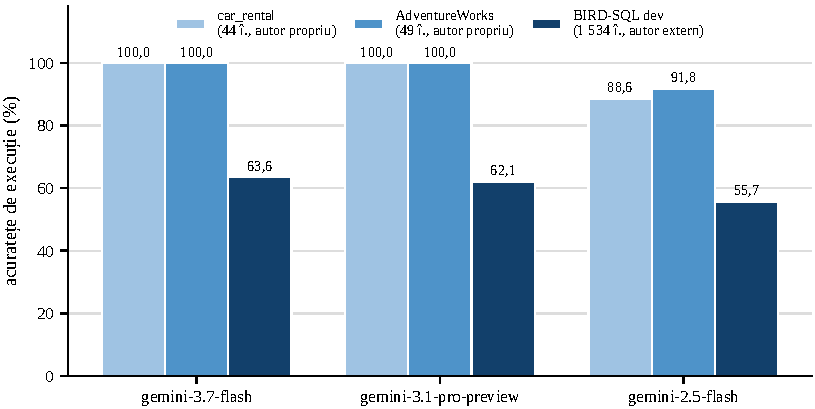
\includegraphics[width=0.95\textwidth]{fig_saturation.pdf}
\caption{Aceleași trei modele, sub aceeași configurație, pe cele trei seturi de
întrebări. Plafonul de performanță (saturația) este depășit prin evaluarea pe baza întrebărilor concepute independent.}
\label{fig:saturare}
\end{figure}

Acesta este rezultatul central al secțiunii, ilustrat în figura~\ref{fig:saturare}, iar scăderea scorurilor absolute
reflectă un beneficiu metodologic, permițând discriminarea obiectivă a sistemelor. Trei modele care pe
întrebările proprii obțineau 100\,\%, deci erau indistinctibile între ele,
coboară pe BIRD într-o bandă de 56--65\,\%, suficient de largă pentru a le
ordona. \textbf{Capacitatea de discriminare a sistemelor a fost restabilită prin utilizarea unui set de
întrebări independent}, și nu prin sporirea complexității sintactice, abordare
care s-a dovedit ineficientă în secțiunea~\ref{sec:config_a}.

Gradientul de dificultate este monoton în fiecare dintre cele patru rulări,
peste etichetele proprii ale BIRD, pe care cadrul de evaluare nu le primește
niciodată. Patru rulări independente care reproduc aceeași ordonare
constituie totodată dovada că modulul de punctare este corect.
Distribuția performanței pe niveluri de dificultate și pe cele 11 baze de date este ilustrată în figura~\ref{fig:bird}.

\begin{figure}[htbp]
\centering
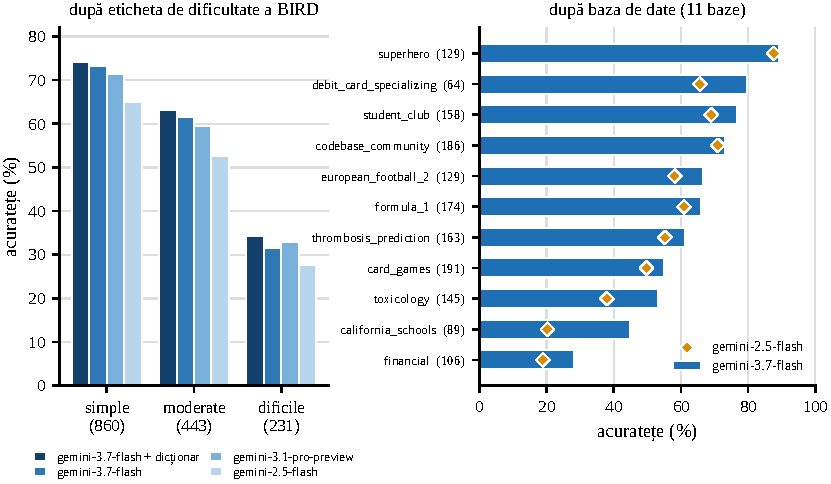
\includegraphics[width=\textwidth]{fig_bird.pdf}
\caption{Stânga: acuratețea pe cele trei niveluri de dificultate ale BIRD.
Dreapta: dispersia pe cele 11 baze de date, cu numărul de întrebări în
paranteză.}
\label{fig:bird}
\end{figure}

\subsection{Comparația de performanță: modelul pro versus modelul flash}

\code{gemini-3.1-pro-preview} obține o acuratețe \emph{inferioară}
modelului \code{gemini-3.7-flash}, la un cost de 5 ori mai ridicat și o latență de 3 ori mai
mare: deși cele două fuseseră indistinctibile pe ambele baze proprii.
Descompunerea pe dificultate explică de ce: modelul pro câștigă +1,3 puncte pe
întrebările \emph{dificile}, dar pierde 2,0 și 2,2 puncte pe cele
\emph{simple} și \emph{moderate}, care reprezintă 85\,\% din set.

Profilul erorilor confirmă această concluzie: modelul pro
produce \textbf{1} interogare invalidă și \textbf{21} de refuzuri, în timp ce
flash produce 12 invalide și 8 refuzuri. Modelul pro manifestă o prudență sporită
(generând refuzuri de răspuns), penalizată mai sever în acuratețea de execuție
decât generarea de sintaxă invalidă de către modelul flash.

Este exact tiparul din secțiunea~\ref{sec:config_b}, reprodus într-un cadru complet diferit: acolo,
Opus 5 (81,8\,\%) se clasa sub Sonnet 5 (93,2\,\%) și sub Haiku 4.5
(84,1\,\%). \textbf{Capacitatea modelului nu ordonează rezultatele, în niciunul
dintre cele două experimente.}

\subsection{Impactul dicționarului de date asupra acurateței}

BIRD livrează un dicționar de date per coloană pe care îl ține deliberat în
afara DDL-ului. În baza \code{financial}, o coloană a cărei linie
\code{CREATE TABLE} conține clauza \code{A3 TEXT not null} are intrarea de dicționar
\emph{„region”}, de neghicit din schemă.

Rulările din tabelul~\ref{tab:bird} folosesc \emph{doar DDL brut}, ceea ce
păstrează contractul de prompt identic cu cel din secțiunea~\ref{sec:config_a}. Rularea suplimentară
adaugă dicționarul de date păstrând neschimbați toți ceilalți parametri, rezultatele fiind sintetizate în tabelul~\ref{tab:dict}:

\begin{table}[H]
\centering
\caption{Efectul dicționarului de date, \code{gemini-3.7-flash}.}
\label{tab:dict}
\footnotesize
\begin{tabular}{@{}lrr@{}}
\toprule
& \hd{Tokeni de prompt} & \hd{Acuratețe} \\
\midrule
DDL brut & 1\,062 & 63,6\,\% \\
DDL + dicționar & 2\,600 & \textbf{64,9\,\%} \\
\bottomrule
\end{tabular}
\end{table}

\textbf{Un spor de +1,3 puncte procentuale obținut cu un prompt de 2,4 ori mai mare.} Efectul nu reprezintă
un câștig pur de precizie: la nivelul fiecărei întrebări, dicționarul
\emph{a corectat 64 de cazuri și a provocat erori în alte 44}, soldul net fiind de +20. Pe baze de date individuale, bilanțul net
ajunge de la $+10$ (\code{toxicology}) și $+5$ (\code{student\_club}), acolo
unde numele coloanelor sunt opace, la $-3$ (\code{financial},
\code{superhero}), acolo unde cei 1\,538 de tokeni suplimentari de proză
aglomerează schema cu informație plauzibilă, dar irelevantă. Pe
\code{card\_games} efectul se anulează exact: dicționarul corectează 9 întrebări
și induce erori în alte 9.

Consecința pentru lucrare este că valoarea de 63,6\,\% se află la mai puțin
de un punct de configurația comparabilă cu clasamentul, deci poate fi citată
alături de cifrele publicate, cu o notă de subsol, iar promptul rămâne
identic cu cel folosit pe celelalte două baze, ceea ce menține toate cele
trei seturi în același experiment.

\subsection{Dispersia între baze de date}

\begin{table}[H]
\centering
\caption{Acuratețea pe fiecare dintre cele 11 baze BIRD.}
\label{tab:birddb}
\footnotesize
\begin{tabular}{@{}lrrrr@{}}
\toprule
\hd{Baza de date} & \hd{Î.} & \hd{3.7-flash} & \hd{3.1-pro} & \hd{2.5-flash} \\
\midrule
\code{superhero} & 129 & 89,1\,\% & 86,0\,\% & 87,6\,\% \\
\code{debit\_card\_specializing} & 64 & 79,7\,\% & 75,0\,\% & 65,6\,\% \\
\code{student\_club} & 158 & 76,6\,\% & 77,2\,\% & 69,0\,\% \\
\code{codebase\_community} & 186 & 73,1\,\% & 74,7\,\% & 71,0\,\% \\
\code{european\_football\_2} & 129 & 66,7\,\% & 64,3\,\% & 58,1\,\% \\
\code{formula\_1} & 174 & 66,1\,\% & 64,9\,\% & 60,9\,\% \\
\code{thrombosis\_prediction} & 163 & 61,3\,\% & 59,5\,\% & 55,2\,\% \\
\code{card\_games} & 191 & 55,0\,\% & 54,5\,\% & 49,7\,\% \\
\code{toxicology} & 145 & 53,1\,\% & 45,5\,\% & 37,9\,\% \\
\code{california\_schools} & 89 & 44,9\,\% & 43,8\,\% & 20,2\,\% \\
\code{financial} & 106 & 28,3\,\% & 28,3\,\% & 18,9\,\% \\
\bottomrule
\end{tabular}

\end{table}

Așa cum reiese din tabelul~\ref{tab:birddb}, dispersia este de 61 de puncte între baze, pe un singur model: mult mai
mare decât cele 8 puncte care separă modelele între ele. \textbf{Particularitățile bazei de date influențează
performanța într-o măsură mai mare decât alegerea modelului.} Baza \code{financial}, la 28,3\,\%, prezintă
cel mai ridicat grad de opacitate al identificatorilor de coloane (\code{A2}, \code{A3}, \code{A11}).

\subsection{Validarea manuală a eșecurilor de execuție}

Un scor de 63,6\,\% pentru un model care atinge 100\,\% pe întrebările
proprii ar putea sugera prezența unor anomalii metodologice în cadrul de evaluare. În consecință,
un eșantion stratificat de 30 de interogări eșuate a fost reexecutat și verificat manual,
fiind clasificat în tabelul~\ref{tab:misses}:

\begin{table}[H]
\centering
\caption{Clasificarea manuală a eșecurilor dintr-un eșantion stratificat.}
\label{tab:misses}
\footnotesize
\begin{tabular}{@{}lr@{}}
\toprule
\hd{Cauză} & \hd{Nr.} \\
\midrule
Răspuns greșit autentic (formă corectă, valori greșite) & 8 \\
Set de coloane greșit / număr de rânduri greșit & 4 \\
SQL-ul modelului nu s-a executat & 1 \\
\textbf{Artefact de punctare} (confirmat drept corect de metrica oficială BIRD) & \textbf{1} \\
\bottomrule
\end{tabular}
\end{table}

Un singur caz din cele 14 eșecuri analizate reprezintă un artefact de punctare. Metrica oficială BIRD
compară \emph{mulțimi} de tupluri; cadrul de evaluare de față compară
\emph{multimulțimi}, deci multiplicitatea rândurilor duplicate contează
pentru cadrul de evaluare de față, dar nu și pentru metrica oficială BIRD. Adoptarea regulii exacte a BIRD mută eșantionul de la
53,3\,\% la 56,7\,\%, o singură întrebare. Aceasta este singura divergență
între cele două metrici și este declarată aici tocmai pentru că afectează
comparabilitatea cu clasamentul.

Celelalte 13 sunt modurile de eșec canonice descrise de autorii BIRD ---
ancorare în valori și literali sensibili la majuscule, nu construcție de SQL:

\begin{lstlisting}[caption={Trei eșecuri reprezentative, cu numărul de rânduri
returnate de fiecare interogare.},captionpos=b]
gold  WHERE A3 = 'north Bohemia'         -> 2260
pred  WHERE A3 = 'North Bohemia'         ->    0   <- 'n' mic in date

gold  WHERE Location = 'New York'        ->   15
pred  WHERE Location LIKE '%New York%'   ->  295

gold  WHERE atom_id LIKE '%_19'          ->  498
pred  WHERE atom_id = '19'               ->    0   <- id-urile sunt TR000_19
\end{lstlisting}

\subsection{Note de metodă}

\begin{itemize}[nosep,leftmargin=*]
  \item \textbf{Toate cele 1\,534 de întrebări sunt incluse}, fără
    eșantionare.
  \item \textbf{Validarea referințelor a rulat prima.} Toate cele 1\,534 de
    interogări de referință au fost executate înainte de orice apel către un
    model. \emph{Niciuna nu returnează zero rânduri}, deci mecanismul de
    refuz al referințelor triviale rămâne armat. Trei depășesc limita de 15 s
    și sunt înregistrate ca eroare de referință, nu ca eșec al modelului;
    reducând scorul fiecărei rulări cu 3 puncte.
  \item \textbf{SQLite, nu tradus.} Interogările de referință BIRD sunt
    scrise pentru SQLite. Portarea lor la PostgreSQL ar fi substituit SQL-ul
    propriu celui al setului de evaluare.
  \item \textbf{Câmpul de cunoaștere externă este inclus}, așa cum cere
    definiția sarcinii din BIRD; întrebările nu sunt rezolvabile fără el.
  \item \textbf{Comparare fără ordine}, conform metricii proprii a BIRD.
\end{itemize}

\section{Amenințări la adresa validității și limitări}
\label{sec:validitate}

\subsection{Anomalii identificate în cadrul de evaluare și remedierea acestora}

Rularea modelelor locale a evidențiat trei anomalii latente. Toate trei
\emph{diminuau acuratețea exclusiv în cazul modelelor locale}: o formă de eroare
sistematică ce risca să conducă la concluzii eronate, acestea fiind sintetizate în tabelul~\ref{tab:defecte}.

\begin{table}[H]
\centering
\caption{Defectele descoperite, efectul lor și remedierea.}
\label{tab:defecte}
\footnotesize
\begin{tabularx}{\textwidth}{@{}p{3.1cm} L L@{}}
\toprule
\hd{Defect} & \hd{Efect} & \hd{Remediere} \\
\midrule
\textbf{Ipoteză asupra formatului de ieșire.} Extractorul de SQL elimina
blocul marcat doar dacă răspunsul \emph{începea} cu el &
Arctic își narează derivarea și pune interogarea într-un bloc \emph{final},
deci întreaga narațiune era executată ca predicție: 0/2 pe întrebări
răspunse corect &
Se ia \emph{ultimul} bloc marcat. Pentru ambele forme produse de modelele din
cloud rezultatul este identic la nivel de octet, rezultatele configurației A
rămânând complet neschimbate \\
\addlinespace
\textbf{Limitarea lungimii de generare clasificată ca eșec al modelului.} Limita de ieșire era de
4\,096 de tokeni &
Un model care raționează înainte de a răspunde consumă cea mai mare parte a
bugetului ajungând la interogare: qwen3.5-9B era trunchiat la 6 din 44 &
Ridicare la 8\,192. \emph{Întregul set de rulări locale a fost reexecutat integral},
asigurând condiții experimentale riguros uniforme pentru toate rezultatele configurației C \\
\addlinespace
\textbf{Trunchierea răspunsului clasificată drept gestiune a ambiguității.} Această configurație calcula
„a cerut clarificare” ca „nu a produs SQL” &
Șase răspunsuri trunchiate erau contorizate drept cereri de clarificare,
denaturând metrica de evaluare a ambiguității &
Detectarea explicită a motivului de oprire, înregistrare separată, excludere
din coloana de clarificări \\
\bottomrule
\end{tabularx}
\end{table}

Fișierele generate anterior acestei remedieri nu includ câmpul respectiv,
absența sa funcționând ca indicator de învechire ce determină excluderea
automată a rulării din agregările curente.

\subsection{Acoperire}

Situația măsurătorilor și a limitelor de acoperire este centralizată în tabelul~\ref{tab:acoperire}.

\begin{table}[H]
\centering
\caption{Sinteza acoperirii experimentale și a limitărilor acesteia.}
\label{tab:acoperire}
\footnotesize
\begin{tabularx}{\textwidth}{@{}L p{4.6cm}@{}}
\toprule
\hd{Celulă} & \hd{Stare} \\
\midrule
Configurație A, 5 modele $\times$ 2 baze & măsurat \\
Configurație B, 7 sisteme, \code{car\_rental} & măsurat \\
Configurație C, 6 modele, \code{car\_rental}; 5 modele, \code{adventureworks} &
măsurat \\
Configurație A, 4 rulări, BIRD-SQL dev (1\,534 î.) & măsurat \\
Configurație B pe \code{adventureworks} & nerulat --- nu se știe dacă penalizarea
agentică crește cu dimensiunea schemei \\
Configurație C pe BIRD & nerulat --- circa 19 ore doar pentru modelul rar \\
\code{claude-agent} pe \code{claude-fable-5} & parțial, exclus (vezi secțiunea~\ref{sec:metodologie_testare}) \\
\textbf{Conducta RAG proprie (configurația din secțiunea~\ref{sec:rag})} &
\textbf{nemăsurată față de setul curent de întrebări}, detaliat în subsecțiunea~\ref{subsec:omisiune_rag} \\
Studiu de varianță pe rulări repetate & învechit \\
\bottomrule
\end{tabularx}
\end{table}

\subsection{Considerații privind evaluarea conductei RAG proprii}
\label{subsec:omisiune_rag}

Conducta RAG descrisă în secțiunea~\ref{sec:rag} \textbf{nu apare în niciun tabel din acest
capitol}. Ultima ei măsurătoare a fost făcută față de un set de întrebări
ulterior înlocuit, iar mecanismul de amprentare o marchează, corect, drept
învechită. Alternativa ar fi fost citarea unei cifre obținute pe alte
întrebări decât cele față de care sunt raportate toate celelalte sisteme, cu
riscul de a sugera o comparabilitate inexistentă.

Această delimitare este asumată explicit în cadrul metodologic: \textbf{lucrarea nu
își propune să demonstreze că soluția proprie depășește cele trei configurații măsurate}. Obiectivul
validat experimental îl constituie analiza comparativă riguroasă dintre arhitecturile de generare,
ale cărei concluzii sunt independente de conducta proprie. Reluarea acestei măsurători este
prima poziție din direcțiile de dezvoltare (secțiunea~\ref{sec:directii_dezvoltare}).

\subsection{Limite cunoscute ale măsurătorii}

\begin{itemize}[nosep,leftmargin=*]
  \item \textbf{Autorul întrebărilor.} Două din cele trei seturi sunt scrise
    de autorul sistemului. Secțiunea~\ref{sec:bird} este contramăsura adoptată.
  \item \textbf{Scara schemelor.} Bazele au 9, 68 și, la BIRD, între 3 și 13
    tabele. Concluziile acestei lucrări nu pot fi extrapolate direct la depozite masive de date
    (sute de tabele), regim studiat de Spider 2.0 \cite{spider2} și
    BEAVER \cite{beaver}.
  \item \textbf{Metrica acceptă răspunsul corect dintr-un motiv greșit.} Compararea
    seturilor de rezultate nu poate diferenția o interogare semantic corectă de una care
    returnează accidental aceleași tupluri.
  \item \textbf{Ambiguitatea este punctată binar} (vezi rezerva din secțiunea~\ref{sec:ambiguitate}).
  \item \textbf{O singură rulare per celulă.} Un studiu anterior de varianță a
    stabilit o dispersie de 3,8 puncte pe șase rulări, dar \emph{pe setul
    vechi de întrebări}. Prin urmare, \textbf{diferențele sub aproximativ 4
    puncte pe 44 de întrebări trebuie tratate ca zgomot} până la refacerea
    acelui studiu. Aceasta nu afectează rezultatele principale, care sunt
    despărțite de 20 până la 45 de puncte, dar afectează ordonarea fină din
    interiorul fiecărei configurații.
\end{itemize}

% =====================================================================
\chapter{Concluzii}
\label{chap:concluzii}
% =====================================================================

\section{Contribuții personale}

\begin{enumerate}[nosep,leftmargin=*]
  \item \textbf{Un cadru de evaluare reproductibil pentru sisteme text-to-SQL},
    care punctează prin execuție reală, izolează o singură variabilă între
    rulări comparate, înregistrează costul alături de acuratețe și își
    detectează singur rulările învechite prin amprentarea setului de
    întrebări. Mecanismul de amprentare și-a dovedit utilitatea practic, prin
    interceptarea unei rulări învechite la generarea figurilor acestei
    lucrări.
  \item \textbf{O măsurătoare a fezabilității accesului agentic la baza de
    date}, sub protocol controlat, peste două \emph{harness}-uri
    independente și șase modele, raportată la două repere obținute în
    aceleași condiții.
  \item \textbf{Două seturi de întrebări construite pe categorii derivate din
    taxonomia de erori publicată în literatură}, incluzând o categorie de
    întrebări deliberat ambigue, punctate pe cererea de clarificare. Spre
    deosebire de seturile dedicate ambiguității \cite{ambiqt, practiq},
    acestea măsoară comportamentul în aceeași rulare cu acuratețea.
  \item \textbf{Un executor cu două motoare} (PostgreSQL și SQLite), care a
    permis validarea externă pe BIRD fără a traduce interogările de referință
    ale setului de evaluare, adică fără a modifica obiectul măsurat.
  \item \textbf{Un sistem funcțional de interogare în limbaj natural}, cu
    conductă de recuperare, validare pe arbore sintactic, execuție
    read-only și generare de rapoarte.
\end{enumerate}

\section{Analiza rezultatelor}

\textbf{Accesul agentic la baza de date funcționează, dar nu la nivelul pe
care îl sugerează argumentul din spatele lui.} Toate configurațiile agentice
măsurate produc interogări corecte pentru majoritatea întrebărilor
(79,5--95,5\,\%), deci abordarea este fezabilă. Niciuna nu atinge însă
reperul obținut cu un singur apel, iar costul este de 9 până la 63 de ori mai
mare. Rezultatul se reproduce peste două \emph{harness}-uri independente,
șase modele și trei furnizori, deci nu este un accident de implementare.
Predicția intuitivă (că un model care poate inspecta baza de date va scrie
interogări mai bune) nu se verifică în condițiile măsurate. O delimitare metodologică importantă este că evaluarea vizează
agentul în configurația sa nativă: datele nu indică o deficiență intrinsecă a modelelor agentice,
ci sugerează că un agent generalist de programare nu este optim adaptat unei sarcini determinate,
rezolvabile mai eficient printr-un apel unic structurat. Disocierea riguroasă a celor două cauze ar necesita un
experiment dedicat care să varieze cadrul de execuție al agentului (\emph{harness}-ul), menținând modelul fixat.

\textbf{Inferența locală este o alternativă viabilă, iar criteriul de selecție
este contraintuitiv.} Un model MoE de 35 de miliarde de parametri, pe o placă
de 12 GiB, egalează cel mai bun agent din familia Claude și depășește
patru dintre cele șapte sisteme agentice. Factorul limitativ nu este
dimensiunea fișierului, ci densitatea arhitecturii: modelul cu cel mai mare volum ocupat pe disc atinge
o viteză de peste șase ori mai mare decât un model dens de dimensiune semnificativ mai mică. Pentru orice
organizație care nu poate trimite date în afara perimetrului propriu, acesta
este rezultatul cu cea mai directă consecință practică.

\textbf{Capacitatea modelului nu ordonează rezultatele.} În configurația agentică,
Opus 5 se clasează sub Sonnet 5 și sub Haiku 4.5; pe BIRD, modelul „pro”
obține un scor inferior modelului „flash”, la un cost de cinci ori mai ridicat. Ambele situații reflectă aceeași
dinamică: modelul cu o capacitate computațională superioară direcționează resursele către prudență decizională
excesivă și explorare redundantă, generând refuzuri nejustificate în detrimentul răspunsurilor exacte.
Alegerea modelului pentru un mediu de producție nu poate fi fundamentată exclusiv pe poziția acestuia în
ierarhia comercială a furnizorului.

\textbf{Un set de evaluare saturat ocultează diferențele dintre sisteme, iar
soluția nu constă în sporirea complexității sintactice a interogărilor.} Cât timp toate modelele obțin 100\,\%, niciun
model nu poate fi declarat superior altuia. Creșterea dificultății
sintactice a întrebărilor proprii nu a schimbat această situație; schimbarea
autorului întrebărilor a schimbat-o imediat, coborând aceleași modele la
56--65\,\% și redând astfel măsurătorii puterea de a le ordona. Mai mult, dispersia de 61 de puncte
între bazele BIRD, față de cele 8 puncte dintre modele, arată că
\emph{domeniul și particularitățile bazei de date} au un impact mai mare asupra performanței finale decât
\emph{alegerea modelului}.

\textbf{Lacuna reală de capacitate este ambiguitatea.} Este singura dimensiune
măsurată care nu s-a saturat. Modelele detectează ambiguitatea explicită și o ratează
sistematic pe cea latentă: la întrebări care par determinate, dar admit mai mulți numitori
apărabili, toate cele cinci modele cu apel unic au ales implicit o variantă fără a solicita
clarificări. Accesul prin unelte inversează acest rezultat, ceea ce
oferă un argument măsurat (singurul din lucrare) în favoarea accesului
la date pentru clarificare, și justifică mecanismul de clarificare din
sistemul propriu.

\section{Direcții de dezvoltare}
\label{sec:directii_dezvoltare}

\begin{enumerate}[nosep,leftmargin=*]
  \item \textbf{Măsurarea conductei RAG proprii față de setul curent de
    întrebări}: singura celulă absentă din capitolul~\ref{chap:rezultate} și, în consecință,
    prima prioritate. Ar permite testarea directă a ipotezei că recuperarea
    curatoriată se comportă diferit de explorarea agentică.
  \item \textbf{Refacerea studiului de varianță} pe setul curent, pentru a
    stabili pragul sub care diferențele nu sunt semnificative.
  \item \textbf{Punctarea ambiguității pe trei stări} (răspuns tăcut, răspuns
    cu ipoteză enunțată explicit, cerere de clarificare), ceea ce ar
    transforma singura dimensiune nesaturată într-o metrică utilizabilă.
  \item \textbf{Extinderea configurației agentice la AdventureWorks}, pentru a
    stabili dacă penalizarea agentică crește sau scade cu dimensiunea schemei.
  \item \textbf{O configurație hibridă}: un singur apel pentru generarea SQL, cu
    unelte disponibile \emph{exclusiv} pentru rezolvarea ambiguității.
    Rezultatele din secțiunile~\ref{sec:config_b} și~\ref{sec:ambiguitate} sugerează împreună că aceasta este configurația
    care combină avantajele fără costul lor.
  \item \textbf{Măsurarea pe scheme de ordinul sutelor de tabele}, regimul în
    care Spider 2.0 \cite{spider2} și BEAVER \cite{beaver} arată că sistemele actuale coboară sub 20\,\% și
    asupra cărora prezenta lucrare nu formulează concluzii empirice.
\end{enumerate}

% =====================================================================
\begin{thebibliography}{99}
\addcontentsline{toc}{chapter}{Bibliografie}

\bibitem{spider}
T. Yu, R. Zhang, K. Yang \emph{et al.}, „Spider: A Large-Scale Human-Labeled
Dataset for Complex and Cross-Domain Semantic Parsing and Text-to-SQL Task”,
în \emph{Proceedings of EMNLP 2018}, Association for Computational
Linguistics, Bruxelles, Belgia, 2018, pp.\ 3911--3921.
\url{https://arxiv.org/abs/1809.08887}

\bibitem{bird}
J. Li, B. Hui, G. Qu \emph{et al.}, „Can LLM Already Serve as A Database
Interface? A BIg Bench for Large-Scale Database Grounded Text-to-SQLs”, în
\emph{Advances in Neural Information Processing Systems 36 (NeurIPS 2023),
Datasets and Benchmarks Track}, New Orleans, SUA, 2023.
\url{https://arxiv.org/abs/2305.03111}

\bibitem{spider2}
F. Lei, J. Chen, Y. Ye \emph{et al.}, „Spider 2.0: Evaluating Language Models
on Real-World Enterprise Text-to-SQL Workflows”, în \emph{Proceedings of the
13th International Conference on Learning Representations (ICLR 2025)},
Singapore, 2025. \url{https://arxiv.org/abs/2411.07763}, consultat în august
2026.

\bibitem{beaver}
P. B. Chen, D. Yang, W. Li \emph{et al.}, „BEAVER: An Enterprise Benchmark
for Text-to-SQL”, preprint arXiv, 2024.
\url{https://arxiv.org/abs/2409.02038}, consultat în august 2026.

\bibitem{brokenbench}
T. Jin, Y. Choi, Y. Zhu și D. Kang, „Text-to-SQL Benchmarks are Broken: An
In-Depth Analysis of Annotation Errors”, în \emph{Proceedings of the
Conference on Innovative Data Systems Research (CIDR 2026)}, Santa Cruz,
SUA, 2026. \url{https://www.vldb.org/cidrdb/papers/2026/p5-jin.pdf},
consultat în august 2026.

\bibitem{deathschema}
K. Maamari, F. Abubaker, D. Jaroslawicz și A. Mhedhbi, „The Death of Schema
Linking? Text-to-SQL in the Age of Well-Reasoned Language Models”, în
\emph{Proceedings of the NeurIPS 2024 Third Table Representation Learning
Workshop}, Vancouver, Canada, 2024.
\url{https://arxiv.org/abs/2408.07702}, consultat în august 2026.

\bibitem{nl2sqlbugs}
X. Liu, S. Shen, B. Li, N. Tang și Y. Luo, „NL2SQL-BUGs: A Benchmark for
Detecting Semantic Errors in NL2SQL Translation”, în \emph{Proceedings of the
31st ACM SIGKDD Conference on Knowledge Discovery and Data Mining}, Toronto,
Canada, 2025. \url{https://arxiv.org/abs/2503.11984}, consultat în august
2026.

\bibitem{arctic}
Z. Yao, G. Sun, L. Borchmann \emph{et al.} (Snowflake AI Research,
University of Maryland, University of California San Diego),
„Arctic-Text2SQL-R1: Simple Rewards, Strong Reasoning in Text-to-SQL”,
preprint arXiv, 2025. \url{https://arxiv.org/abs/2505.20315}, consultat în
august 2026.

\bibitem{mcp}
Agentic AI Foundation (protocol inițiat de Anthropic în 2024, donat
fundației în decembrie 2025), „Model Context Protocol --- Specification
(2025-06-18)”, documentație tehnică on-line.
\url{https://modelcontextprotocol.io/specification/2025-06-18}, consultat în
august 2026.

\bibitem{mcpbench}
Z. Luo, X. Shi, X. Lin și J. Gao, „Evaluation Report on MCP Servers”,
preprint arXiv, 2025. \url{https://arxiv.org/abs/2504.11094}, consultat în
septembrie 2026.

\bibitem{dailsql}
D. Gao, H. Wang, Y. Li \emph{et al.}, „Text-to-SQL Empowered by Large Language
Models: A Benchmark Evaluation”, în \emph{Proceedings of the VLDB Endowment},
vol.\ 17, nr.\ 5, 2024, pp.\ 1132--1145.
\url{https://www.vldb.org/pvldb/vol17/p1132-gao.pdf}, consultat în septembrie
2026.

\bibitem{ambiqt}
A. Bhaskar, T. Tomar, A. Sathe și S. Sarawagi, „Benchmarking and Improving
Text-to-SQL Generation under Ambiguity”, în \emph{Proceedings of the 2023
Conference on Empirical Methods in Natural Language Processing (EMNLP)},
Singapore, 2023, pp.\ 7053--7074.
\url{https://arxiv.org/abs/2310.13659}, consultat în septembrie 2026.

\bibitem{practiq}
M. Dong, N. A. Kumar, Y. Hu \emph{et al.}, „PRACTIQ: A Practical
Conversational Text-to-SQL Dataset with Ambiguous and Unanswerable Queries”,
preprint arXiv, 2024. \url{https://arxiv.org/abs/2410.11076}, consultat în
septembrie 2026.

\bibitem{birdleaderboard}
BIRD-SQL, „Leaderboard”, clasament on-line actualizat continuu.
\url{https://bird-bench.github.io/}, consultat în august 2026.

\bibitem{claudecode}
Anthropic, „Claude Code, agentic coding tool”, documentație de produs
on-line. \url{https://claude.com/product/claude-code}, consultat în august
2026.

\bibitem{codexcli}
OpenAI, „Codex CLI --- coding agent that runs in your terminal”,
documentație de produs on-line.
\url{https://developers.openai.com/codex/cli/}, consultat în august 2026.

\bibitem{postgresql}
PostgreSQL Global Development Group, „PostgreSQL --- documentație oficială”.
\url{https://www.postgresql.org/docs/}, consultat în august 2026.

\bibitem{sqlite}
SQLite Consortium, „SQLite: documentație oficială”.
\url{https://www.sqlite.org/docs.html}, consultat în august 2026.

\bibitem{aaif}
Linux Foundation, „Linux Foundation Announces the Formation of the Agentic AI
Foundation (AAIF), Anchored by New Project Contributions Including Model
Context Protocol (MCP), goose and AGENTS.md”, comunicat de presă, decembrie
2025.
\url{https://www.linuxfoundation.org/press/linux-foundation-announces-the-formation-of-the-agentic-ai-foundation},
consultat în septembrie 2026.

\bibitem{transformer}
A. Vaswani, N. Shazeer, N. Parmar \emph{et al.}, „Attention Is All You Need”,
în \emph{Advances in Neural Information Processing Systems 30 (NIPS 2017)},
Long Beach, SUA, 2017, pp.\ 5998--6008.
\url{https://arxiv.org/abs/1706.03762}

\bibitem{birddata}
BIRD-SQL, „bird\_sql\_dev\_20251106: revizia setului de dezvoltare”,
HuggingFace Datasets.
\url{https://huggingface.co/datasets/birdsql/bird_sql_dev_20251106},
consultat în august 2026.

\bibitem{advworks}
Microsoft, „AdventureWorks sample databases”; portare PostgreSQL:
NorfolkDataSci, \emph{adventure-works-postgres}, revizia
\code{afcfd2df}. \url{https://github.com/NorfolkDataSci/adventure-works-postgres},
consultat în august 2026.

\bibitem{llamacpp}
G. Gerganov \emph{et al.}, „llama.cpp --- LLM inference in C/C++”, proiect
open-source. \url{https://github.com/ggml-org/llama.cpp}, consultat în august
2026.

\bibitem{pgserver}
O. Moll, „pgserver, embedded PostgreSQL server for Python”, Python Package
Index. \url{https://pypi.org/project/pgserver/}, consultat în august 2026.

\bibitem{qwen}
Alibaba Cloud, „Qwen3.5 și Qwen3.6, carduri de model”, documentație de
produs; fără raport tehnic publicat la data redactării. Fișierele GGUF
efectiv măsurate provin de la doi cuantizatori terți,
\code{lmstudio-community} și \code{unsloth}, identificați prin numele exact
al depozitului HuggingFace în anexa~\ref{anx:modele}. Consultat în august
2026.

\end{thebibliography}

% =====================================================================
\appendix
\renewcommand{\thechapter}{\Alph{chapter}}
\addcontentsline{toc}{chapter}{Anexe}

\chapter{Modelele măsurate}
\label{anx:modele}

Cuantizarea este parte a măsurătorii.
De aceea fiecare model local este identificat prin fișierul
exact rulat.

\begin{table}[H]
\centering
\footnotesize
\caption{Modelele locale, cu fișierul GGUF măsurat.}
\begin{tabularx}{\textwidth}{@{}p{4.3cm} L@{}}
\toprule
\hd{Model} & \hd{Fișier GGUF} \\
\midrule
Arctic-Text2SQL-R1-7B \cite{arctic} &
\code{mradermacher/Arctic-Text2SQL-R1-7B-GGUF}, \code{Q4\_K\_M} (4,4 GiB) și
\code{Q8\_0} (7,5 GiB) \\
Qwen3.5-9B \cite{qwen} &
\code{lmstudio-community/Qwen3.5-9B-GGUF}, \code{Q4\_K\_M} (5,2 GiB) \\
Qwen3.6-27B (dens) &
\code{unsloth/Qwen3.6-27B-GGUF}, \code{UD-IQ3\_XXS} (11,2 GiB) \\
Qwen3.6-35B-A3B (MoE, activare parțială) &
\code{unsloth/Qwen3.6-35B-A3B-GGUF}, \code{UD-Q4\_K\_M} (20,6 GiB) \\
Bonsai-27B &
\code{lmstudio-community/Bonsai-27B-GGUF}, \code{Q1\_0} (3,5 GiB). Metadatele
GGUF nu conțin legătură \code{base\_model}: partajează arhitectura
Qwen3.6-27B, dar nu este o cuantizare a acestuia \\
\bottomrule
\end{tabularx}
\end{table}

Modelele din cloud sunt produse comerciale fără lucrări publicate. Ele sunt
citate prin identificator și prin tariful în vigoare la momentul rulării
(\code{prices\_checked} 2026-08-23), înregistrat în fiecare fișier de
rezultate.

\begin{table}[H]
\centering
\footnotesize
\caption{Modelele din cloud măsurate.}
\begin{tabularx}{\textwidth}{@{}p{2.0cm} L p{2.5cm}@{}}
\toprule
\hd{Furnizor} & \hd{Modele} & \hd{Folosite în} \\
\midrule
Google &
\code{gemini-2.5-flash}, \code{gemini-3-flash-preview},
\code{gemini-3.1-pro-preview}, \code{gemini-3.6-flash},
\code{gemini-3.7-flash} & configurație A (secțiunea~\ref{sec:config_a}), BIRD (secțiunea~\ref{sec:bird}) \\
Anthropic &
\code{claude-opus-5}, \code{claude-sonnet-5}, \code{claude-haiku-4-5},
\code{claude-fable-5} & configurație B, \code{claude-agent} (secțiunea~\ref{sec:config_b}) \\
OpenAI &
\code{gpt-5.6-sol}, \code{gpt-5.6-terra}, \code{gpt-5.6-luna} &
configurație B, \code{codex-agent} (secțiunea~\ref{sec:config_b}) \\
\bottomrule
\end{tabularx}
\end{table}

\chapter{Reproducerea rezultatelor}
\label{anx:reproducere}

Fiecare cifră din capitolul~\ref{chap:rezultate} este citită din \code{benchmark/results/*.json}
de scripturile care generează tabelele și figurile. Niciun număr nu este
transcris manual.

\begin{lstlisting}[language=bash,caption={Comenzile care regenerează
măsurătorile și materialul grafic al lucrării.},captionpos=b]
# tabelele si figurile din capitolul 4
python docs/diploma/figures/make_all.py

# o rulare a bratului A
python benchmark/run.py --arm naive --model gemini-3.7-flash
python benchmark/run.py --arm naive --model gemini-3.7-flash \
       --dataset adventureworks

# BIRD-SQL dev: construirea setului din cele doua artefacte upstream,
# cu validarea fiecarei interogari de referinta, apoi rularea
python benchmark_data/bird/prepare.py
./benchmark/sweep_bird.sh                 # 3 modele, in paralel
DATASET=bird_dev_dict ./benchmark/sweep_bird.sh gemini-3.7-flash

# bratul local: lista modelelor, pornirea unuia, apoi sweep-ul complet
./benchmark/serve_local.sh --list
./benchmark/serve_local.sh qwen36-35b-moe
./benchmark/sweep_local.sh
\end{lstlisting}

Fiecare fișier de rezultate înregistrează configurația, modelul, amprenta setului
de întrebări, SQL-ul per întrebare, consumul de tokeni per întrebare și
latența, ceea ce permite repunctarea fără reapelarea modelelor.

\section*{Structura seturilor de întrebări}
\addcontentsline{toc}{section}{Structura seturilor de întrebări}

Setul \code{car\_rental} conține 51 de întrebări (44 punctate, 7 ambigue), dintre
care 6 formulate în limba română. Setul \code{adventureworks} conține 56 de
întrebări (49 punctate, 7 ambigue), dintre care 5 în limba română. Distribuția
pe categorii este dată în tabelul~\ref{tab:categorii}; amprentele criptografice
ale celor două seturi sunt \code{86e194123bb3}, respectiv \code{5398f281a907},
iar cea a setului BIRD-SQL dev este \code{e700eb224701}.

Categoriile marcate ca adăugate în etapa a doua au fost introduse după ce
măsurătorile inițiale au arătat că grupurile \emph{simple}, \emph{agregare},
\emph{join} și \emph{subinterogare} încetaseră să diferențieze sistemele din
configurațiile A și B --- motivația introducerii acestora este documentată în
secțiunea~\ref{sec:dificultate}.

\end{document}
